\documentclass[11pt,letterpaper]{article}
\usepackage[utf8]{inputenc}
\usepackage[spanish,es-nodecimaldot]{babel}
\usepackage{amsmath}
\usepackage{amsfonts}
\usepackage{amssymb}
\usepackage{color,soul}
\usepackage{textcomp}
\usepackage{stmaryrd}
\usepackage{makeidx}
\newcommand{\xmark}{\ding{55}}%
\usepackage{pifont}% http://ctan.org/pkg/pifont

\usepackage{colortbl}
\usepackage{tocloft}
\renewcommand{\cftsecleader}{\cftdotfill{\cftdotsep}}
\usepackage{rotating}
\usepackage{url}
\usepackage{pdflscape} 
\usepackage{pdfpages}
\usepackage{float}
\usepackage{graphicx}
\usepackage{ marvosym }
\usepackage{pgf,tikz}
\usepackage{mathrsfs}
\usetikzlibrary{arrows}
\usepackage{ mathrsfs }
 \usepackage{array}
\usepackage{longtable}
\newcommand{\justif}[2]{&{#1}&\text{#2}}
\usepackage{listings}
\usepackage{color}
\newcolumntype{L}[1]{>{\raggedright\let\newline\\\arraybackslash\hspace{0pt}}m{#1}}
\newcolumntype{C}[1]{>{\centering\let\newline\\\arraybackslash\hspace{0pt}}m{#1}}
\newcolumntype{R}[1]{>{\raggedleft\let\newline\\\arraybackslash\hspace{0pt}}m{#1}}
\definecolor{dkgreen}{rgb}{0,0.6,0}
\definecolor{gray}{rgb}{0.5,0.5,0.5}
\definecolor{mauve}{rgb}{0.58,0,0.82}
\setboolean{@twoside}{false}
\lstset{frame=tb,
  language=Java,
  aboveskip=3mm,
  belowskip=3mm,
  showstringspaces=false,
  columns=flexible,
  basicstyle={\small\ttfamily},
  numbers=left,
  numberstyle=\tiny\color{gray},
  keywordstyle=\color{blue},
  commentstyle=\color{dkgreen},
  stringstyle=\color{mauve},
  breaklines=true,
  breakatwhitespace=true,
  tabsize=3
}

\usetikzlibrary{graphs,graphs.standard}
\newcommand{\floor}[1]{\lfloor #1 \rfloor}

\usepackage{multicol}

\usepackage{caption}
\usepackage{subcaption}
\begin{document}
\begin{titlepage}
	\centering
	{\scshape\LARGE Universidad Nacional Autónoma de México \par}
	\vspace{1cm}
	{\scshape\Large Facultad de Ciencias\par}
	\vspace{1.5cm}
\begin{center}
		
\includegraphics[scale=.5]{logo.png}
	\end{center}
		\vspace{.8 cm}

	{\huge\bfseries Proyecto Final: \par}
	{\huge\bfseries Normalización del Modelo \par}
		\vspace{0.5cm}

	{\Large\itshape Flores Martínez Andrés\\
	Vázquez Salcedo Eduardo Eder\\
	Sánchez Pérez Pedro Juan Salvador\\
	Concha Vázquez Miguel\par}
	\vfill
			\vspace{0.5cm}

	Trabajo presentado en cumplimiento con la asignatura de Fundamentos de Bases de Datos impartida por el profesor	\par
	 \textsc{Gerardo Avilés Rosas}\\
	\vspace{0.1cm}
	{\large 12 de enero de 2018\par}
\end{titlepage}

\begin{center}
\tableofcontents
\end{center}

\newpage

Con tal de acabar, en la medida de lo posible, con las anomalías como son la redundancia de la información, procederemos a normalizar el diseño. Frecuentemente para ésto recurriremos a la descomposición de relaciones, pasando paulatinamente del cumplimiento de la serie de reglas de las distintas formas normales. En nuestro caso, luego de haber normalizado a primera y segunda forma normal continuaremos directamente con la normalización a forma normal de Boyce-Codd; esto se debe a que como revisamos en el curso, la última está contenida en la tercera forma normal, así que por consiguiente también lo habremos normalizado a tercera forma normal\footnote{De cualquier manera agregamos en la última sección la normalización que correspondería a normalizar a tercera forma normal en caso de que hubiera alguna pérdida de dependencias funcionales al tratar de normalizar a BCNF, lo cual no fue el caso.}. \\

Para poder llevar a cabo la técnica de normalización desarrollada por Edgar Frank Codd en el año de 1972, primeramente vamos a tener que identificar las dependencias funcionales existentes en nuestras relaciones, recordando para ésto que son relaciones unidireccionales entre dos atributos de tal forma que si ocurre que $X\rightarrow Y$ (El conjunto de atributos $X$ determina funcionalmente al conjunto de atributos $Y$) en un momento dado ocurre que para cada valor único de $X$ sólo un valor de $Y$ se asocia con él a través de la relación. En nuestro caso no identificamos dependencias multivaluadas al ocuparnos desde un inicio en la normalización a primera forma normal del tener dominios atómicos y atributos no multivaluados en las tablas, por lo que no requeriremos un normalización a cuarta forma normal (4NF). 
\begin{center}
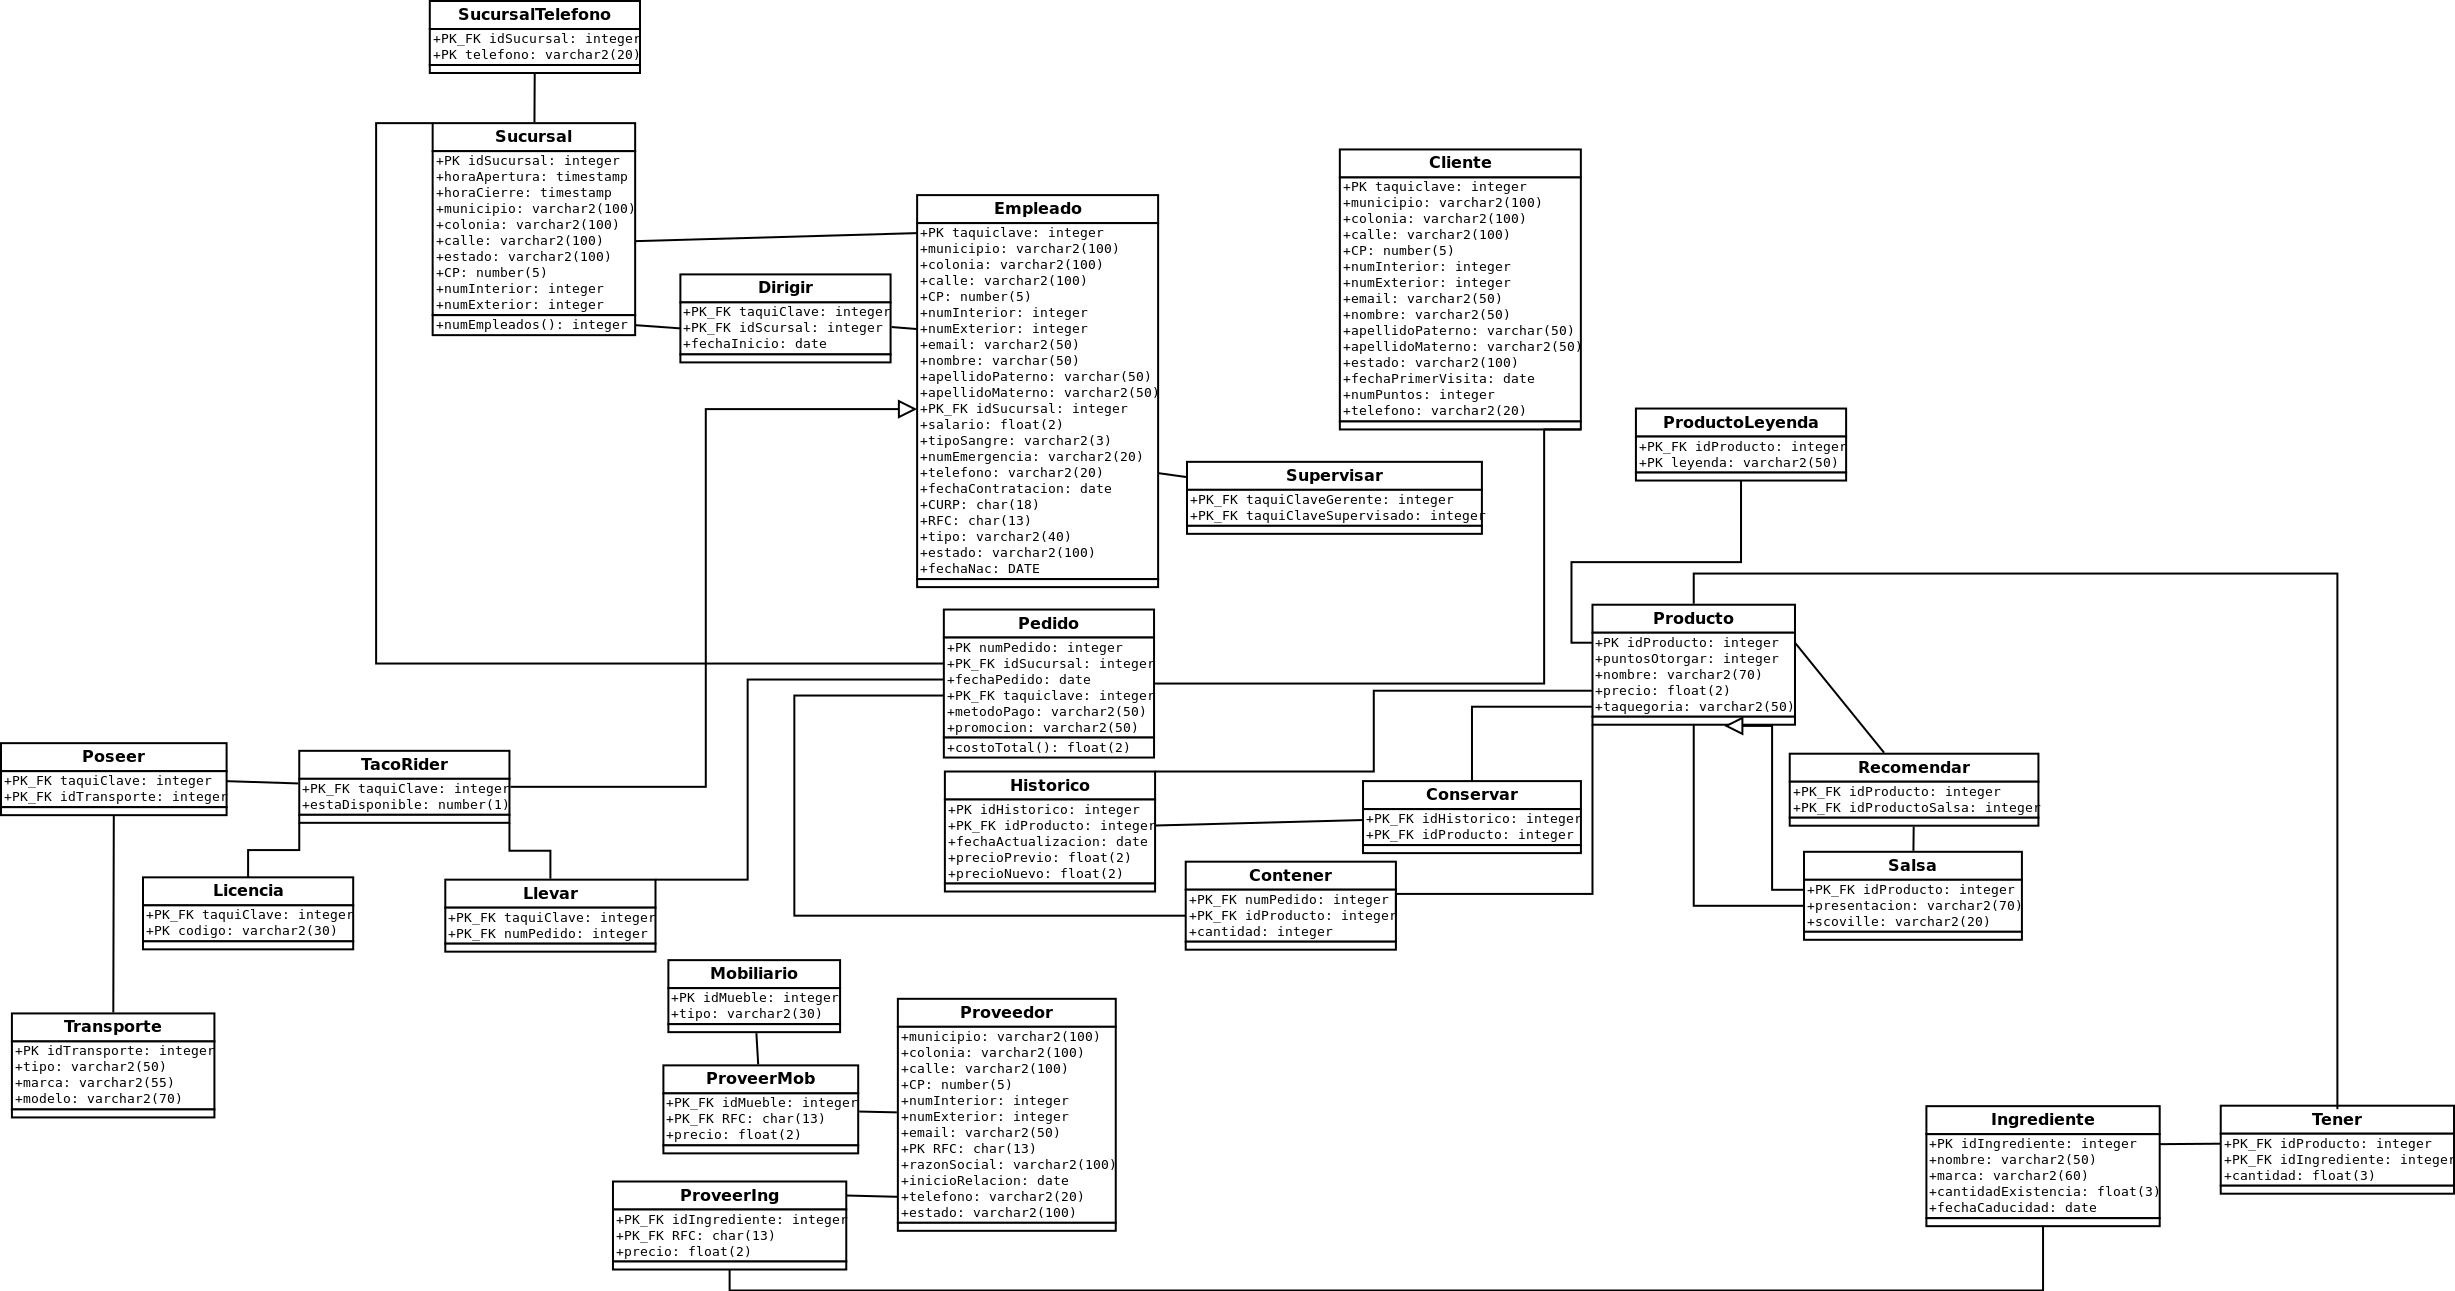
\includegraphics[width=\linewidth]{UML_no_normalizado.png}
\captionof{figure}{Consideremos el UML para iniciar el proceso de normalización.}
\end{center}



\section{Primera Forma Normal (1NF)}

\subsection{Proceso de Normalización}

Para que las relaciones se encuentren en \textit{primera formal normal}, todos los atributos deberán ser \textbf{atómicos}, esto es, asegurar que las columnas de la tabla no sean multivaluadas (que no contengan más de un valor del dominio para una misma tupla). Además, debemos asegurar que:

\begin{itemize}
\item No haya orden de arriba hacia abajo, ni de izquierda a derecha en cuanto a los dominios y a los atributos.
\item Que no se tengan registros (tuplas) duplicadas.
\item Que cada celda de nuestra tabla tenga exactamente un solo valor de un dominio.
\end{itemize}

Como en el proceso de traducción (transformación) del diagrama Entidad-Relación ya nos aseguramos de que los atributos multivaluados se vieran transformados en nuevas relaciones cuyo atributo llave era el nombre mismo del atributo multivaluado y con una llave externa (llave foránea) con el atributo llave de la entidad de la cual eran atributos multivaluados, ya aseguramos que ninguna de nuestras tuplas de toda relación de nuestro modelos tiene valores multivaluados.\\

Por otro lado, tal como se ilustra en el ejemplo de la práctica actual, también es menester para llevar las relaciones del modelo a la \textit{primer forma normal} el hecho de asegurar que cada registro (tupla) no almacene información multivaluada de diversos dominios.\\

Vamos a revisar cada tabla (relación) del modelo previo para verificar si ya se encuentra o no en la forma normal de interés actualmente:

\begin{itemize}
\item \textbf{Categoría}: Los atributos de la tabla ya poseen dominios atómicos, es decir, que no pueden ser separados en dominios más pequeños. En consecuencia, ya se encuentra en \textit{primera forma normal}.
\item \textbf{Cliente}: Los atributos que eran susceptibles de tener dominios no atómicos ya están separados, como es el caso de todos los datos correspondientes a la dirección del cliente y los de su nombre. Además, la fecha no necesita ser separada en día, mes y año porque el manejador de la base de datos puede trabajar sobre el tipo \textit{DATE} que contempla los tres campos mencionados. Por ende, ya se encuentra en \textit{primera forma normal}.
\item \textbf{Conservar}: Como es una relación que hace referencia a atributos llave de otras relaciones cuyos dominios no pueden ser separados (son llaves foráneas), entonces la relación ya está en \textit{primera forma normal}.
\item \textbf{Contener}: Ocurre exactamente lo mismo que en el caso previo al hacer referencia a llaves atómicas de otras tablas. En cuento al atributo \textit{cantidad}, es ya atómico al ser un entero. Por tanto, la relación (tabla) se encuentra ya en \textit{primera forma normal}.
\item \textbf{Dirigir}: Como ha ocurrido previamente, el único atributo candidato a ser violación a la primer forma normal es el de la \textit{fechaInicio}, pues los otros son llaves foráneas que por medio de la política de llaves externas hacen referencia a las llaves de otras tablas, mismos atributos que ya tienen un dominio atómico. La fecha ---como ya se mencionó en el caso de la relación (tabla) \textbf{Cliente}--- no nos conviene separarla en día, mes y año porque contamos en el dato de tipo \textit{DATE}. Así, vemos que ya está en \textit{primera forma normal}.
\item \textbf{Empleado}: Ocurre en este caso algo parecido a la relación de \textbf{Cliente} porque originalmente era también una sub-entidad de la entidad fuerte \textbf{Persona} del formalismo provisto por el diagrama entidad-relación. En consecuencia, hemos ya separado los dominios no atómicos de la dirección desde un inicio al considerarlo como un atributo compuesto, lo mismo que en el caso del nombre del empleado. Todos los demás atributos no son candidatos a ser violación de la forma normal al tener dominios atómicos. Se sigue entonces que está ya en \textit{primer forma normal}.

\item \textbf{Histórico}: No es posible dividir más los dominios de sus registros,
así que se encuentra ya en \textit{primera forma normal.}
\item \textbf{Ingrediente}: Todos los dominios de los atributos de la relación son ya atómicos, por lo que cumple con estar en \textit{primera forma normal.}
\item \textbf{Licencia}: La \textit{taquiClave} es una llave foránea que es llave primaria a de la tabla \textbf{TacoRider}, misma que posee un dominio atómico. El único otro atributo es el código de la licencia, pero puede ser expresado por medio del tipo \textit{varchar2}\footnote{El tipo \textit{varchar} está ya en desuso.}, así que sus dominios son atómicos y se encuentra en \textit{primera forma normal}.
\item \textbf{Llevar}: Sus dos atributos son llaves foráneas de las tablas \textbf{TacoRider} y \textbf{Pedido}, que tienen atómicos los dominios de sus llaves. Se sigue entonces que la relación está ya en \textit{primera forma normal}.
\item \textbf{Mobiliario}:

\item \textbf{Pedido}: Ningún atributo tiene dominios que no sean atómicos, por lo que entonces ya se encuentra en \textit{primera forma normal}.
\item \textbf{Poseer}: Los dos atributos de la relación (tabla) son llaves foráneas de otras tablas en la que los atributos cuentan con un dominio atómico. Por ende, la relación está ya en \textit{primera forma normal}.
\item \textbf{Producto}: No es posible dividir más los dominios de sus registros, así
que se encuentra ya en \textit{primera forma normal}.
\item \textbf{ProductoLeyenda}: No es posible dividir más los dominios de sus registros, así
que se encuentra ya en \textit{primera forma normal}.
\item \textbf{Proveedor}: El único dato que sería susceptible de ser violación a la forma normal es el que corresponde a la dirección del proveedor, pero ya fue correctamente manejado en sus componentes constituyentes desde el diagrama entidad-relación. Así, ya se encuentra en \textit{primera forma normal}.

\item \textbf{ProveerIng}: Esta relación posee dos atributos que son llaves externas; los atributos llave de las tablas a las que se hace referencia poseen dominios atómicos. En cuanto al atributo de \textit{precio}, posee ya un dominio que es atómico. Por lo mencionado anteriormente se sigue que esta relación se encuentra ya en \textit{primera forma normal}.
\item \textbf{ProveerMob}: Lo que ocurre en este caso es análogo a la relación previa; así, se encuentra de entrada en \textit{primera forma normal}.
\item \textbf{Recomendar}: Los dos atributos de la relación son llaves foráneas que hacen referencia a llaves de otras tablas con dominios atómicos. Entonces, la relación se encuentra ya en \textit{primera forma normal}.
\item \textbf{Salsa}: Los tres atributos de la relación nos son candidatos a ser violaciones de la forma normal en cuestión al tener atómicos sus dominios. Por tanto se encuentra en \textit{primera forma normal}. 
\item \textbf{Sucursal}: Los datos correspondientes a la dirección de las sucursales fueron separados por medio de un atributo compuesto desde la formalización presentada en el diagrama entidad-relación, así que tienen dominios atómicos. Más aún, hicimos una distinción explícita entre la hora de inicio y término de las clases. Por ende, se encuentra la relación en \textit{primera forma normal}.

\item \textbf{SucursalTelefono}: No es posible dividir más los dominios de sus registros, así que se encuentra ya en \textit{primera forma normal}.
\item \textbf{Supervisar}: Sus dos atributos son llaves foráneas que hacen referencia a la \textit{taquiClave} de la relación \textbf{Empleado}. Dicho atributo llave posee un dominio atómico y entonces se encuentra ya en \textit{primera forma normal}.
\item \textbf{TacoRider}: Sus dos atributos tienen atómicos sus dominios; se encuentra ya en \textit{primera forma normal}.
\item \textbf{Tener}: Esta relación (tabla) tiene dos atributos que son llave foránea. Los atributos entonces hacen referencia a llaves de las tablas \textbf{Producto} e \textbf{Ingrediente} que poseen dominios atómicos. El atributo de \textit{cantidad} también posee un dominio que es atómico al no poder ser separado más. Así, la relación cumple ya con el hecho de estar en \textit{primer forma normal}.
\item \textbf{Transporte}:No es posible dividir más los dominios de sus registros, así que se encuentra ya en \textit{primera forma normal}.
\end{itemize}

Con todo esto, obtuvimos el mismo resultado porque ya estaba en \textit{primera forma normal} nuestro modelo.

\subsection{Relaciones Generadas}
\begin{itemize}
\item \footnotesize{\textbf{Categoría}(\underline{idProducto},taquegoria)}
\item \footnotesize{\textbf{Cliente}(\underline{taquiClave},email,telefono,nombre,apellidoPaterno,apellidoMaterno,calle,municipio,colonia,estado,
numInterior,numExterior,CP,numPuntos,fechaPrimerVisita)}
\item \footnotesize{\textbf{Conservar}(\underline{idHistorico},\underline{idProducto})}
\item \footnotesize{\textbf{Contener}(\underline{numPedido},\underline{idProducto},cantidad)}
\item \footnotesize{\textbf{Dirigir}(\underline{taquiClave},\underline{idSucursal},fechaInicio)}
\item \footnotesize{\textbf{Empleado}(\underline{taquiClave},email,telefono,nombre,apellidoPaterno,apellidoMaterno,calle,municipio,colonia,estado,
numInterior,numExterior,CP,CURP,RFC,tipo,tipoSangre,fechaNac,fechaContratacion,
numEmergencia,salario,\underline{idSucursal})}
\item \footnotesize{\textbf{Historico}(\underline{idHistorico},idProducto,precioPrevio,precioNuevo,fechaActualizacion)}
\item \footnotesize{\textbf{Ingrediente}(\underline{idIngrediente},nombre,marca,cantidadExistencia,fechaCaducidad)}
\item \footnotesize{\textbf{Licencia}(\underline{codigo},\underline{taquiClave}})
\item \footnotesize{\textbf{Llevar}(\underline{numPedido},\underline{taquiClave})}
\item \footnotesize{\textbf{Mobiliario}(\underline{idMueble},tipo)}
\item \footnotesize{\textbf{Pedido}(\underline{numPedido},fechaPedido,promocion,preparado,entregado,\underline{taquiClave},metodoPago,\underline{idSucursal})}
\item \footnotesize{\textbf{Poseer}(\underline{taquiClave},\underline{idTransporte})}
\item \footnotesize{\textbf{Producto}(\underline{idProducto},nombre,precio,taquegoria,descripcion)}
\item \footnotesize{\textbf{ProductoLeyenda}(\underline{idProducto},\underline{leyenda})}
\item \scriptsize{\textbf{Proveedor}(\underline{RFC},razonSocial,calle,municipio,colonia,estado,numInterior,numExterior,CP,email,inicioRelacion,telefono)}
\item \footnotesize{\textbf{ProveerIng}(\underline{RFC},\underline{idIngrediente},precio)}
\item \footnotesize{\textbf{ProveerMob}(\underline{RFC},\underline{idMueble},precio)}
\item \footnotesize{\textbf{Recomendar}(\underline{idProducto},\underline{idProductoSalsa})}
\item \footnotesize{\textbf{Salsa}(\underline{idProducto},scoville,presentacion)}
\item {\footnotesize \textbf{Sucursal}(\underline{idSucursal},calle,municipio,colonia,estado,numInterior,numExterior,CP,horaApertura,horaCierre)}
\item \footnotesize{\textbf{SucursalTelefono}(\underline{idSucursal},\underline{telefono})}
\item \footnotesize{\textbf{Supervisar}(\underline{taquiClaveGerente},\underline{taquiClaveSupervisado})}
\item \footnotesize{\textbf{TacoRider}(\underline{taquiClave},estaDisponible)}
\item \footnotesize{\textbf{Tener}(\underline{idProducto},\underline{idIngrediente},cantidad)}
\item \footnotesize{\textbf{Transporte}(\underline{idTransporte},marca,modelo,tipo)}



\end{itemize}
\subsection{Diagrama de Clases UML}

\begin{landscape}
\begin{center}
\begin{minipage}{1\linewidth}
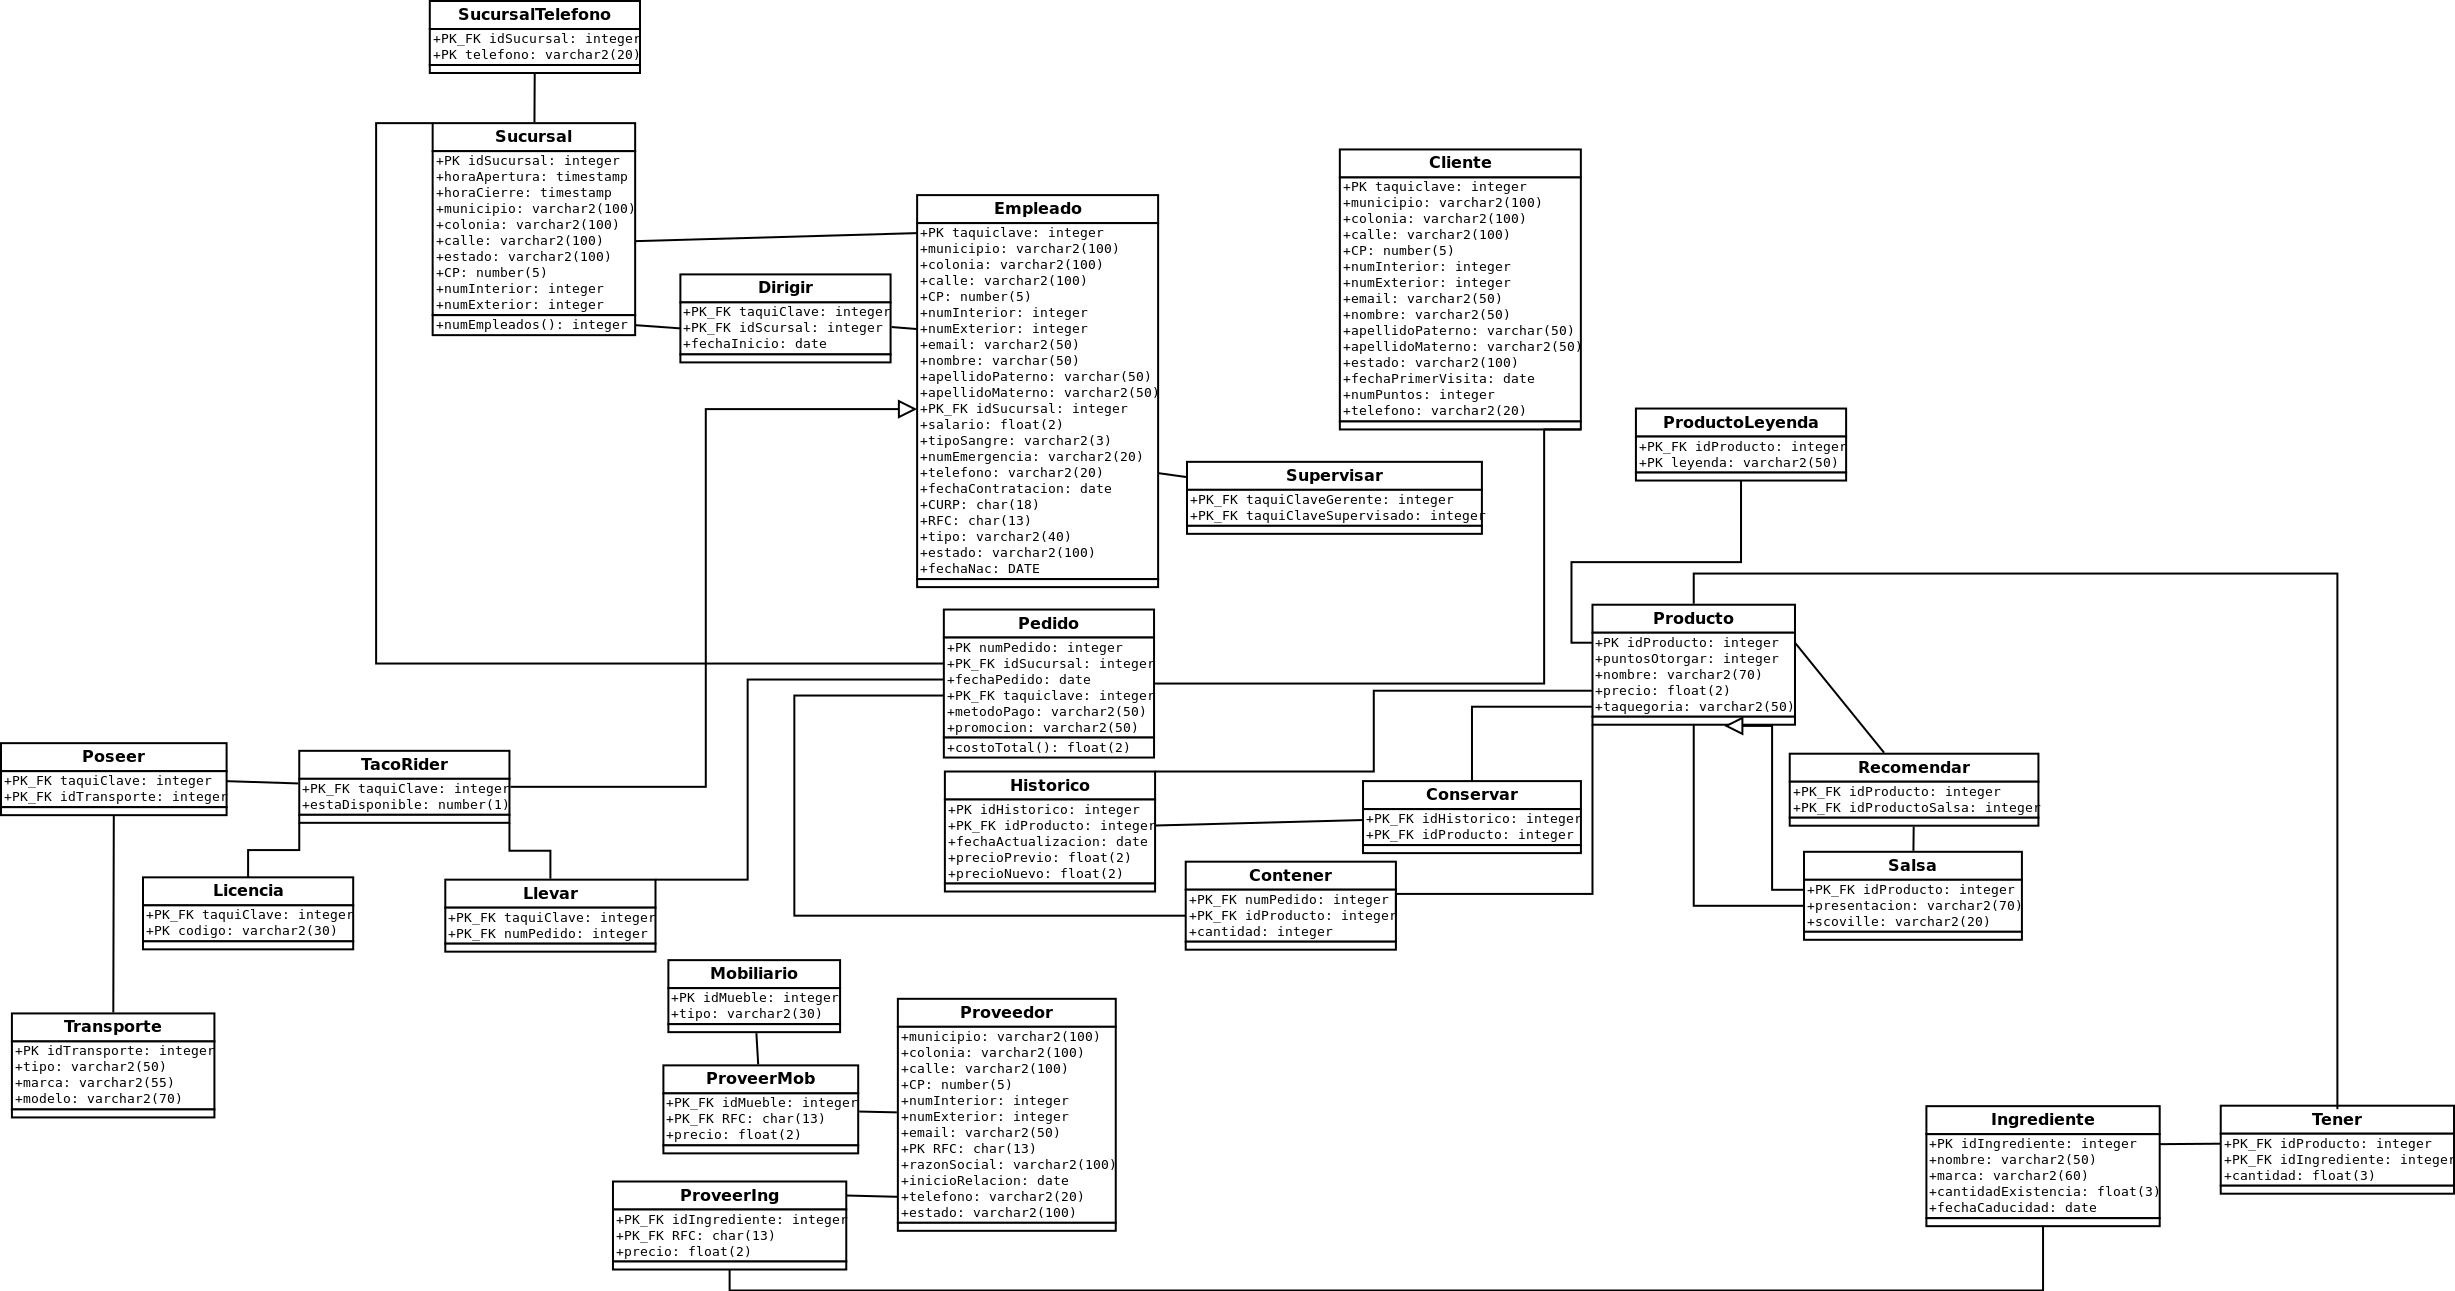
\includegraphics[width=\linewidth]{1NF.png}
\captionof{figure}{Modelo en primera forma normal.}
\end{minipage}
\end{center}
\end{landscape}

%%%%%%%%%%%%%%%%%%%%%%%%%%%%%%%%%%%%%%%
\section{Segunda Forma Normal (2NF)}

\subsection{Proceso de Normalización}

A partir de este punto, comenzaremos a usar las dependencias funcionales de las relaciones para lograr la normalización, factor que no incidía en la normalización a \textit{primera forma normal}. \\

De acuerdo con la teoría, una relación estará en \textit{segunda forma normal} en caso de que todo atributo no llave depende del atributo llave de la relación. En los casos en que esto regla no se cumpla para algún atributo de la relación, lo que suele hacerse es separar la información que se encuentra determinada funcionalmente por un atributo que no es llave primaria. A continuación, consideremos las dependencias funcionales de nuestras relaciones en \textit{primera forma normal} y a partir de ello evaluaremos si están o no en \textit{segunda forma normal}. En caso de presentarse violaciones, procederemos a normalizar.

\begin{itemize}

\item \textbf{Categoría}: Tenemos las dependencias funcionales que siguen:

\begin{itemize}
\item idProducto $\rightarrow$ idProducto

\item idProducto $\rightarrow$ taquegoría
\end{itemize}

Evidentemente todo atributo no llave (en este caso la llave débil o discriminante de \textit{taquegoría}) depende funcionalmente de la llave de la tabla, que en este caso es \textit{idProducto}. Por ende, ya se encuentra normalizada a \textit{segunda forma normal}. 

\item \textbf{Cliente}: Tenemos las dependencias funcionales que siguen:

\begin{itemize}
\item taquiClave $\rightarrow$ taquiClave

\item taquiClave $\rightarrow$ email
\item taquiClave $\rightarrow$ telefono
\item taquiClave $\rightarrow$ nombre
\item taquiClave $\rightarrow$ apellidoPaterno
\item taquiClave $\rightarrow$ apellidoMaterno
\item taquiClave $\rightarrow$ municipio
\item taquiClave $\rightarrow$ colonia
\item taquiClave $\rightarrow$ calle
\item taquiClave $\rightarrow$ CP
\item taquiClave $\rightarrow$ numInterior
\item taquiClave $\rightarrow$ numExterior
\item taquiClave $\rightarrow$ estado
\item taquiClave $\rightarrow$ fechaPrimerVisita
\item taquiClave $\rightarrow$ numPuntos
\item CP $\rightarrow$ estado
\end{itemize}

Donde la última es debido a que dos códigos postales no pueden ser iguales y corresponder a dos estados distintos de la República Mexicana. \\

Vemos que claramente todo atributo no llave depende de la \textit{taquiClave}, siendo ésta el atributo llave de la relación. Así, está ya en \textit{segunda forma normal}.
\item \textbf{Conservar}: Ya se encuentra en segunda forma normal, pues contamos con una superllave conformada por los dos atributos de llave foránea \textit{idProducto} e \textit{idHistorico} y contamos entonces solamente con la DF trivial:

\begin{itemize}
\item idHistorico idProducto $\rightarrow$ idHistorico \item idProducto
\end{itemize}

Luego, por la regla de inferencia de Arsmtrong de la descomposición tenemos:

\begin{itemize}
\item idHistorico idProducto $\rightarrow$ idHistorico\\
\item idHistorico idProducto $\rightarrow$ idProducto
\end{itemize}


Por tanto, como todo atributo de la relación depende de la llave de la misma ---en este caso compuesta--- la relación cumple con estar ya en \textit{segunda forma normal}.
\item \textbf{Contener}: De manera similar tenemos que la llave de la relación está conformada por sus dos llaves foráneas \textit{numPedido} e \textit{idProducto}. Por tanto, se tiene la dependencia funcional trivial, además de que la llave compuesta determina funcionalmente a la cantidad de cada producto usado en cada pedido. Por tanto, tenemos las siguientes DFs\footnote{A partir de este punto vamos a aplicar en diversas ocasiones la regla de inferencia de Armstrong de la descomposición, por lo cual omitiremos la explicación explícita de la separación de los atributos dependientes de las DFs.}:

\begin{itemize}
\item numPedido idProducto $\rightarrow$ numPedido idProducto

\item numPedido idProducto $\rightarrow$ numPedido
\item numPedido idProducto $\rightarrow$ idProducto
\item numPedido idProducto $\rightarrow$ cantidad
\end{itemize}

Como todo atributo no llave depende funcionalmente de la llave de la relación (tabla), entonces cumple con estar en \textit{segunda forma normal}.
\item \textbf{Dirigir}: Nuevamente ocurre que contamos con una llave compuesta por ambas llaves foráneas \textit{taquiClave} e \textit{idSucursal}; contamos entonces con la dependencia funcional trivial y como no puede ser que para una misma combinación de una clave de empleado con una de sucursal se asocien dos fechas de inicio distintas, tenemos también que \textit{fechaInicio} está determinada funcionalmente por la llave compuesta. Tenemos entonces las siguientes dependencias funcionales:

\begin{itemize}
\item taquiClave idSucursal $\rightarrow$ taquiClave idSucursal

\item taquiClave idSucursal $\rightarrow$ taquiClave
\item taquiClave idSucursal $\rightarrow$ idSucursal
\item taquiClave idSucursal $\rightarrow$ fechaInicio
\end{itemize}

Dado que todo atributo no llave de la relación queda determinado funcionalmente por la llave de la misma, entonces está ya en \textit{segunda forma normal}.
\item \textbf{Empleado}: Ya está en \textit{segunda forma normal}. Se tienen las siguientes dependencias funcionales en la relación:

\begin{itemize}
\item taquiClave $\rightarrow$ taquiClave

\item taquiClave $\rightarrow$ idSucursal
\item taquiClave $\rightarrow$ salario 
\item taquiClave $\rightarrow$ email
\item taquiClave $\rightarrow$ telefono
\item taquiClave $\rightarrow$ nombre
\item taquiClave $\rightarrow$ apellidoPaterno
\item taquiClave $\rightarrow$ apellidoMaterno
\item taquiClave $\rightarrow$ municipio
\item taquiClave $\rightarrow$ colonia
\item taquiClave $\rightarrow$ calle 
\item taquiClave $\rightarrow$ CP
\item taquiClave $\rightarrow$ numeroInterior
\item taquiClave $\rightarrow$ numeroExterior
\item taquiClave $\rightarrow$ estado
\item taquiClave $\rightarrow$ CURP
\item taquiClave $\rightarrow$ tipoSangre
\item taquiClave $\rightarrow$ numEmergencia
\item taquiClave $\rightarrow$ fechaNac
\item taquiClave $\rightarrow$ tipo 
\item taquiClave $\rightarrow$ RFC
\item taquiClave $\rightarrow$ fechaContratacion
\item CP $\rightarrow$ estado
\item CURP $\rightarrow$ fechaNac
\end{itemize}

En donde la última se tiene porque no puede haber dos CURPS iguales a los que les corresponde distinta fecha de nacimiento.\\

Como ocurre que todo atributo no llave de la relación depende funcionalmente de la llave de ésta, entonces ocurre que está ya en \textit{segunda forma normal}. 

\item \textbf{Histórico}: Contamos con las siguientes dependencias funcionales:

\begin{itemize}
\item idHistorico $\rightarrow$ idHistorico

\item idHistorico $\rightarrow$ idProducto
\item idHistorico $\rightarrow$ fechaActualizacion
\item idHistorico $\rightarrow$ precioPrevio
\item idHistorico $\rightarrow$ precioNuevo
\end{itemize}

Vemos que todos los atributos no llave de la relación dependen funcionalmente de la llave; por ende, está ya en \textit{segunda forma normal}.  

\item \textbf{Ingrediente}: Por cuestiones legales, podemos pensar que el nombre de un ingrediente no puede repetirse, así que podríamos considerarlo como una llave candidata. Tenemos entonces las siguientes dependencias funcionales:

\begin{itemize}
\item idIngrediente $\rightarrow$ idIngrediente

\item idIngrediente $\rightarrow$ nombre
\item idIngrediente $\rightarrow$ marca
\item idIngrediente $\rightarrow$ cantidadExistencia
\item idIngrediente $\rightarrow$ fechaCaducidad

%%

\item nombre $\rightarrow$ nombre

\item nombre $\rightarrow$ idIngrediente
\item nombre $\rightarrow$ marca
\item nombre $\rightarrow$ cantidadExistencia
\item nombre $\rightarrow$ fechaCaducidad
\end{itemize}

Se cumple con la condición de la forma normal que establece que todo atributo no llave debe depender funcionalmente de la llave de la relación (tabla). Por tanto, está ya en \textit{segunda forma normal}. 
\item \textbf{Licencia}: La dependencias funcionales son:

\begin{itemize}
\item codigo $\rightarrow$ codigo

\item codigo $\rightarrow$ taquiClave
\end{itemize}

Se cumple que todo atributo no llave de la relación (aunque en este caso es una llave foránea) depende de la llave de la misma. Por tanto, se encuentra en \textit{segunda forma normal}. 

\item \textbf{Llevar}: La relación tiene como únicos dos atributos a llaves foráneas, así que la llave es compuesta por \textit{taquiClave} y \textit{numPedido}. Entonces, las dependencias funcionales con que se cuenta son:

\begin{itemize}
\item taquiClave numPedido $\rightarrow$ taquiClave numPedido

\item taquiClave numPedido $\rightarrow$ taquiClave
\item taquiClave numPedido $\rightarrow$ numPedido
\end{itemize}

Vemos que todos atributo no llave de la relación dependen funcionalmente de la llave, así que está en \textit{segunda forma normal}. 
\item \textbf{Mobiliario}: La únicas dependencias funcionales que hay son las siguientes:


\begin{itemize}
\item idMueble $\rightarrow$ idMueble

\item idMueble $\rightarrow$ tipo
\end{itemize}

Todo atributo no llave depende funcionalmente de la llave. Por ende, está ya en \textit{segunda forma normal}.

\item \textbf{Pedido}: Está ya en \textit{segunda forma normal}. Las dependencias funcionales son:

\begin{itemize}
\item numPedido $\rightarrow$ numPedido

\item numPedido $\rightarrow$ idSucursal
\item numPedido $\rightarrow$ fechaPedido
\item numPedido $\rightarrow$ taquiClave
\item numPedido $\rightarrow$ metodoPago
\item numPedido $\rightarrow$ promocion
\item numPedido $\rightarrow$ preparado
\item numPedido $\rightarrow$ entregado
\item fechaPedido $\rightarrow$ promocion
\end{itemize}

De donde la última se tiene porque las promociones de la taquería están basadas en los días de la semana, así que no puede ser que para una misma fecha se tengan promociones diferentes; al conocer la fecha del pedido, sabemos el día de la semana y en consecuencia la promoción que fue aplicada.\\

Como todos los atributos no llave de la relación dependen funcionalmente de la llave de la misma, entonces está ya en \textit{segunda forma normal}.
\item \textbf{Poseer}: La llave de la relación está compuesta por ambas llaves foráneas \textit{taquiClave} e \textit{idTransporte}. Entonces, las dependencias funcionales son:

\begin{itemize}
\item taquiClave idTransporte $\rightarrow$ taquiClave idTransporte

\item taquiClave idTransporte $\rightarrow$ taquiClave
\item taquiClave idTransporte $\rightarrow$ idTransporte
\end{itemize}

Se cumple que todo atributo no llave de la relación está determinado funcionalmente por la misma. Así, está ya en \textit{segunda forma normal}.

\item \textbf{Producto}: Ya está en \textit{segunda forma normal}. Las dependencias funcionales son:

\begin{itemize}
\item idProducto $\rightarrow$ idProducto

\item idProducto $\rightarrow$ nombre
\item idProducto $\rightarrow$ precio
\item idProducto $\rightarrow$ descripcion
\item nombre $\rightarrow$ nombre

\item nombre $\rightarrow$ idProducto
\item nombre $\rightarrow$ nombre
\item nombre $\rightarrow$ precio
\item nombre $\rightarrow$ descripcion

\end{itemize}

Vemos nuevamente que tenemos las últimas DFs dado que no puede repetirse el nombre de un producto dentro de la taquería. Entonces, al ser una llave candidata, genera las mismas DFs que la llave de la relación (tabla).\\

Ocurre que todas los atributos no llave de la relación dependen funcionalmente de la llave de esta.
\item \textbf{ProductoLeyenda}: Está en \textit{segunda forma normal} porque todos los atributos no llave de la relación, que en este caso es solamente \textit{leyenda} e \textit{idProducto}, dependen funcionalmente de la llave compuesta\textit{idProducto leyenda}. Esto se ve a partir de las dos DFs con que se cuenta:

\begin{itemize}
\item idProducto leyenda $\rightarrow$ idProducto leyenda

\item idProducto leyenda $\rightarrow$ idProducto
\item idProducto leyenda $\rightarrow$ leyenda

\end{itemize}
\item \textbf{Proveedor}: Las dependencias funcionales que se tienen son:


\begin{itemize}
\item RFC $\rightarrow$ RFC

\item RFC $\rightarrow$ razonSocial
\item RFC $\rightarrow$ inicioRelacion
\item RFC $\rightarrow$ email
\item RFC $\rightarrow$ telefono
\item RFC $\rightarrow$ municipio
\item RFC $\rightarrow$ colonia
\item RFC $\rightarrow$ calle
\item RFC $\rightarrow$ CP
\item RFC $\rightarrow$ numeroInterior
\item RFC $\rightarrow$ numeroExterior
\item RFC $\rightarrow$ estado
\item CP $\rightarrow$ estado

\end{itemize}

Vemos que todos los atributos no llave dependen de esta, así que está ya en \textit{segunda forma normal}.

\item \textbf{ProveerIng}: Las dependencias funcionales son:

\begin{itemize}
\item RFC idIngrediente $\rightarrow$ RFC idIngrediente

\item RFC idIngrediente $\rightarrow$ RFC 
\item RFC idIngrediente $\rightarrow$ idIngrediente
\item RFC idIngrediente $\rightarrow$ precio
\end{itemize}

Como la llave de la relación es una superllave compuesta por \textit{RFC} e \textit{idIngrediente}, se cumple que todos los atributos no llave están determinados funcionalmente por dicha llave y, así, está en \textit{segunda forma normal}.

\item \textbf{ProveerMob}: Ocurre que ---como la relación previa--- está ya en \textit{segunda forma normal}. Las dependencias funcionales que se tienen son:

\begin{itemize}
\item RFC idMueble $\rightarrow$ RFC idMueble

\item RFC idMueble $\rightarrow$ RFC 
\item RFC idMueble $\rightarrow$ idMueble
\item RFC idMueble $\rightarrow$ precio
\end{itemize}

Así, todos los atributos no llave de la relación quedan determinados funcionalmente por la misma.
\item \textbf{Recomendar}: La llave de la relación está compuesta por ambas llaves foráneas \textit{idProducto} e \textit{idProductoSalsa}. Las dependencias funcionales son:

\begin{itemize}
\item idProducto idProductoSalsa $\rightarrow$ idProducto idProductoSalsa

\item idProducto idProductoSalsa $\rightarrow$ idProducto 
\item idProducto idProductoSalsa $\rightarrow$ idProductoSalsa

\end{itemize}

Así, está en \textit{segunda forma normal} dado que todo atributo no llave está determinado funcionalmente por la superllave.
\item \textbf{Salsa}: Como ya ha ocurrido con los ingredientes y los productos, el nombre de una salsa determina funcionalmente a los demás atributos al ser una llave candidata. Así, contamos con las siguientes DFs:

\begin{itemize}
\item idProducto $\rightarrow$ idProducto 

\item idProducto $\rightarrow$ nombre
\item idProducto $\rightarrow$ presentacion
\item idProducto $\rightarrow$ scoville

%%

\item nombre $\rightarrow$ nombre 

\item nombre $\rightarrow$ idProducto
\item nombre $\rightarrow$ presentacion
\item nombre $\rightarrow$ scoville

\end{itemize}

Como todos los atributos no llave de la relación quedan determinados funcionalmente por esta, está ya en \textit{segunda forma normal}. 
\item \textbf{Sucursal}: Las dependencias funcionales que se tienen para esta tabla son:

\begin{itemize}
\item idSucursal $\rightarrow$ idSucursal

\item idSucursal $\rightarrow$ horaApertura
\item idSucursal $\rightarrow$ horaCierre
\item idSucursal $\rightarrow$ municipio
\item idSucursal $\rightarrow$ colonia
\item idSucursal $\rightarrow$ calle
\item idSucursal $\rightarrow$ CP
\item idSucursal $\rightarrow$ numInterior
\item idSucursal $\rightarrow$ numExterior
\item idSucursal $\rightarrow$ estado
\item CP $\rightarrow$ estado

\end{itemize}

Como se cumple que todo atributo no llave está determinado funcionalmente por la llave de la relación, entonces cumple con estar en \textit{segunda forma normal}.
\item \textbf{SucursalTelefono}: La llave de la relación se constituye por \textit{telefono}. Las DFs son:

\begin{itemize}
\item telefono $\rightarrow$ telefono

\item telefono  $\rightarrow$ idSucursal

\end{itemize}

Pues dado un teléfono, no puede ser que haya otra sucursal dentro de la República Mexicana con el mismo número.\\

Entonces, todo atributo no llave de la relación dependen funcionalmente de la llave que se tiene en este escenario y cumple por consiguiente con estar ya en \textit{segunda forma normal}.
\item \textbf{Supervisar}: La relación (tabla) cumple con estar en \textit{segunda forma normal} como vemos a partir de sus dependencias funcionales y viendo que la llave es superllave compuesta por \textit{taquiClaveGerente} y \textit{taquiClaveSupervisado}:

\begin{itemize}
\item taquiClaveGerente taquiClaveSupervisado $\rightarrow$ taquiClaveGerente taquiClaveSupervisado

\item taquiClaveGerente taquiClaveSupervisado $\rightarrow$ taquiClaveGerente 
\item taquiClaveGerente taquiClaveSupervisado $\rightarrow$ taquiClaveSupervisado

\end{itemize}

Entonces, todo atributo no llave depende funcionalmente de la llave de la relación.
\item \textbf{TacoRider}: Las dependencias funcionales que se tienen son:
\begin{itemize}
\item taquiClave $\rightarrow$ taquiClave

\item taquiClave $\rightarrow$ estaDisponible
\end{itemize}

Como todo atributo no llave depende de la llave, ya se encuentra en \textit{segunda forma normal}.
\item \textbf{Tener}: La llave de la relación es compuesta y está constituida por los atributos \textit{idProducto} e \textit{idIngrediente}. Las DFs son:

\begin{itemize}
\item idProducto idIngrediente $\rightarrow$ idProducto idIngrediente

\item idProducto idIngrediente $\rightarrow$ idProducto
\item idProducto idIngrediente $\rightarrow$ idIngrediente

\item idProducto idIngrediente $\rightarrow$ cantidad

\end{itemize}

Donde la última se tiene porque conocido el producto y el ingrediente, es posible determinar qué cantidad de dicho ingrediente fue utilizado en la preparación del producto, i.e., para un mismo producto e ingrediente, no puede corresponder en tuplas distintas una cantidad diferente. \\

Como se cumple que todo atributo no llave dependen funcionalmente de la llave, entonces ya está en \textit{segunda forma normal}.
\item \textbf{Transporte}: Ya está en \textit{segunda forma normal} dado que todos los atributos no llave dependen de la llave \textit{idTransporte} como notamos a partir de la consideración de las DFs de la relación (tabla):

\begin{itemize}
\item idTransporte $\rightarrow$ idTransporte

\item idTransporte $\rightarrow$ tipo
\item idTransporte $\rightarrow$ marca
\item idTransporte $\rightarrow$ modelo
\end{itemize}
\end{itemize}

Notemos que nuevamente no tuvimos que efectuar cambios en el modelo: estaba ya en \textit{segunda forma normal}.

\subsection{Relaciones Generadas}

\begin{itemize}
\item \footnotesize{\textbf{Categoría}(\underline{idProducto},taquegoria)}
\item \footnotesize{\textbf{Cliente}(\underline{taquiClave},email,telefono,nombre,apellidoPaterno,apellidoMaterno,calle,municipio,colonia,estado,
numInterior,numExterior,CP,numPuntos,fechaPrimerVisita)}
\item \footnotesize{\textbf{Conservar}(\underline{idHistorico},\underline{idProducto})}
\item \footnotesize{\textbf{Contener}(\underline{numPedido},\underline{idProducto},cantidad)}
\item \footnotesize{\textbf{Dirigir}(\underline{taquiClave},\underline{idSucursal},fechaInicio)}
\item \footnotesize{\textbf{Empleado}(\underline{taquiClave},email,telefono,nombre,apellidoPaterno,apellidoMaterno,calle,municipio,colonia,estado,
numInterior,numExterior,CP,CURP,RFC,tipo,tipoSangre,fechaNac,fechaContratacion,
numEmergencia,salario,\underline{idSucursal})}
\item \footnotesize{\textbf{Historico}(\underline{idHistorico},idProducto,precioPrevio,precioNuevo,fechaActualizacion)}
\item \footnotesize{\textbf{Ingrediente}(\underline{idIngrediente},nombre,marca,cantidadExistencia,fechaCaducidad)}
\item \footnotesize{\textbf{Licencia}(\underline{codigo},\underline{taquiClave}})
\item \footnotesize{\textbf{Llevar}(\underline{numPedido},\underline{taquiClave})}
\item \footnotesize{\textbf{Mobiliario}(\underline{idMueble},tipo)}
\item \footnotesize{\textbf{Pedido}(\underline{numPedido},fechaPedido,promocion,preparado,entregado,\underline{taquiClave},metodoPago,\underline{idSucursal})}
\item \footnotesize{\textbf{Poseer}(\underline{taquiClave},\underline{idTransporte})}
\item \footnotesize{\textbf{Producto}(\underline{idProducto},nombre,precio,taquegoria)}
\item \footnotesize{\textbf{ProductoLeyenda}(\underline{idProducto,leyenda})}
\item \scriptsize{\textbf{Proveedor}(\underline{RFC},razonSocial,calle,municipio,colonia,estado,numInterior,numExterior,CP,email,inicioRelacion,telefono)}
\item \footnotesize{\textbf{ProveerIng}(\underline{RFC},\underline{idIngrediente},precio)}
\item \footnotesize{\textbf{ProveerMob}(\underline{RFC},\underline{idMueble},precio)}
\item \footnotesize{\textbf{Recomendar}(\underline{idProducto},\underline{idProductoSalsa})}
\item \footnotesize{\textbf{Salsa}(\underline{idProducto},scoville,presentacion)}
\item {\footnotesize \textbf{Sucursal}(\underline{idSucursal},calle,municipio,colonia,estado,numInterior,numExterior,CP,horaApertura,horaCierre)}
\item \footnotesize{\textbf{SucursalTelefono}(\underline{idSucursal},\underline{telefono})}
\item \footnotesize{\textbf{Supervisar}(\underline{taquiClaveGerente},\underline{taquiClaveSupervisado})}
\item \footnotesize{\textbf{TacoRider}(\underline{taquiClave},estaDisponible)}
\item \footnotesize{\textbf{Tener}(\underline{idProducto},\underline{idIngrediente},cantidad)}
\item \footnotesize{\textbf{Transporte}(\underline{idTransporte},marca,modelo,tipo)}



\end{itemize}


\subsection{Diagrama de Clases UML} 

\begin{landscape}
\begin{center}
\begin{minipage}{1\linewidth}
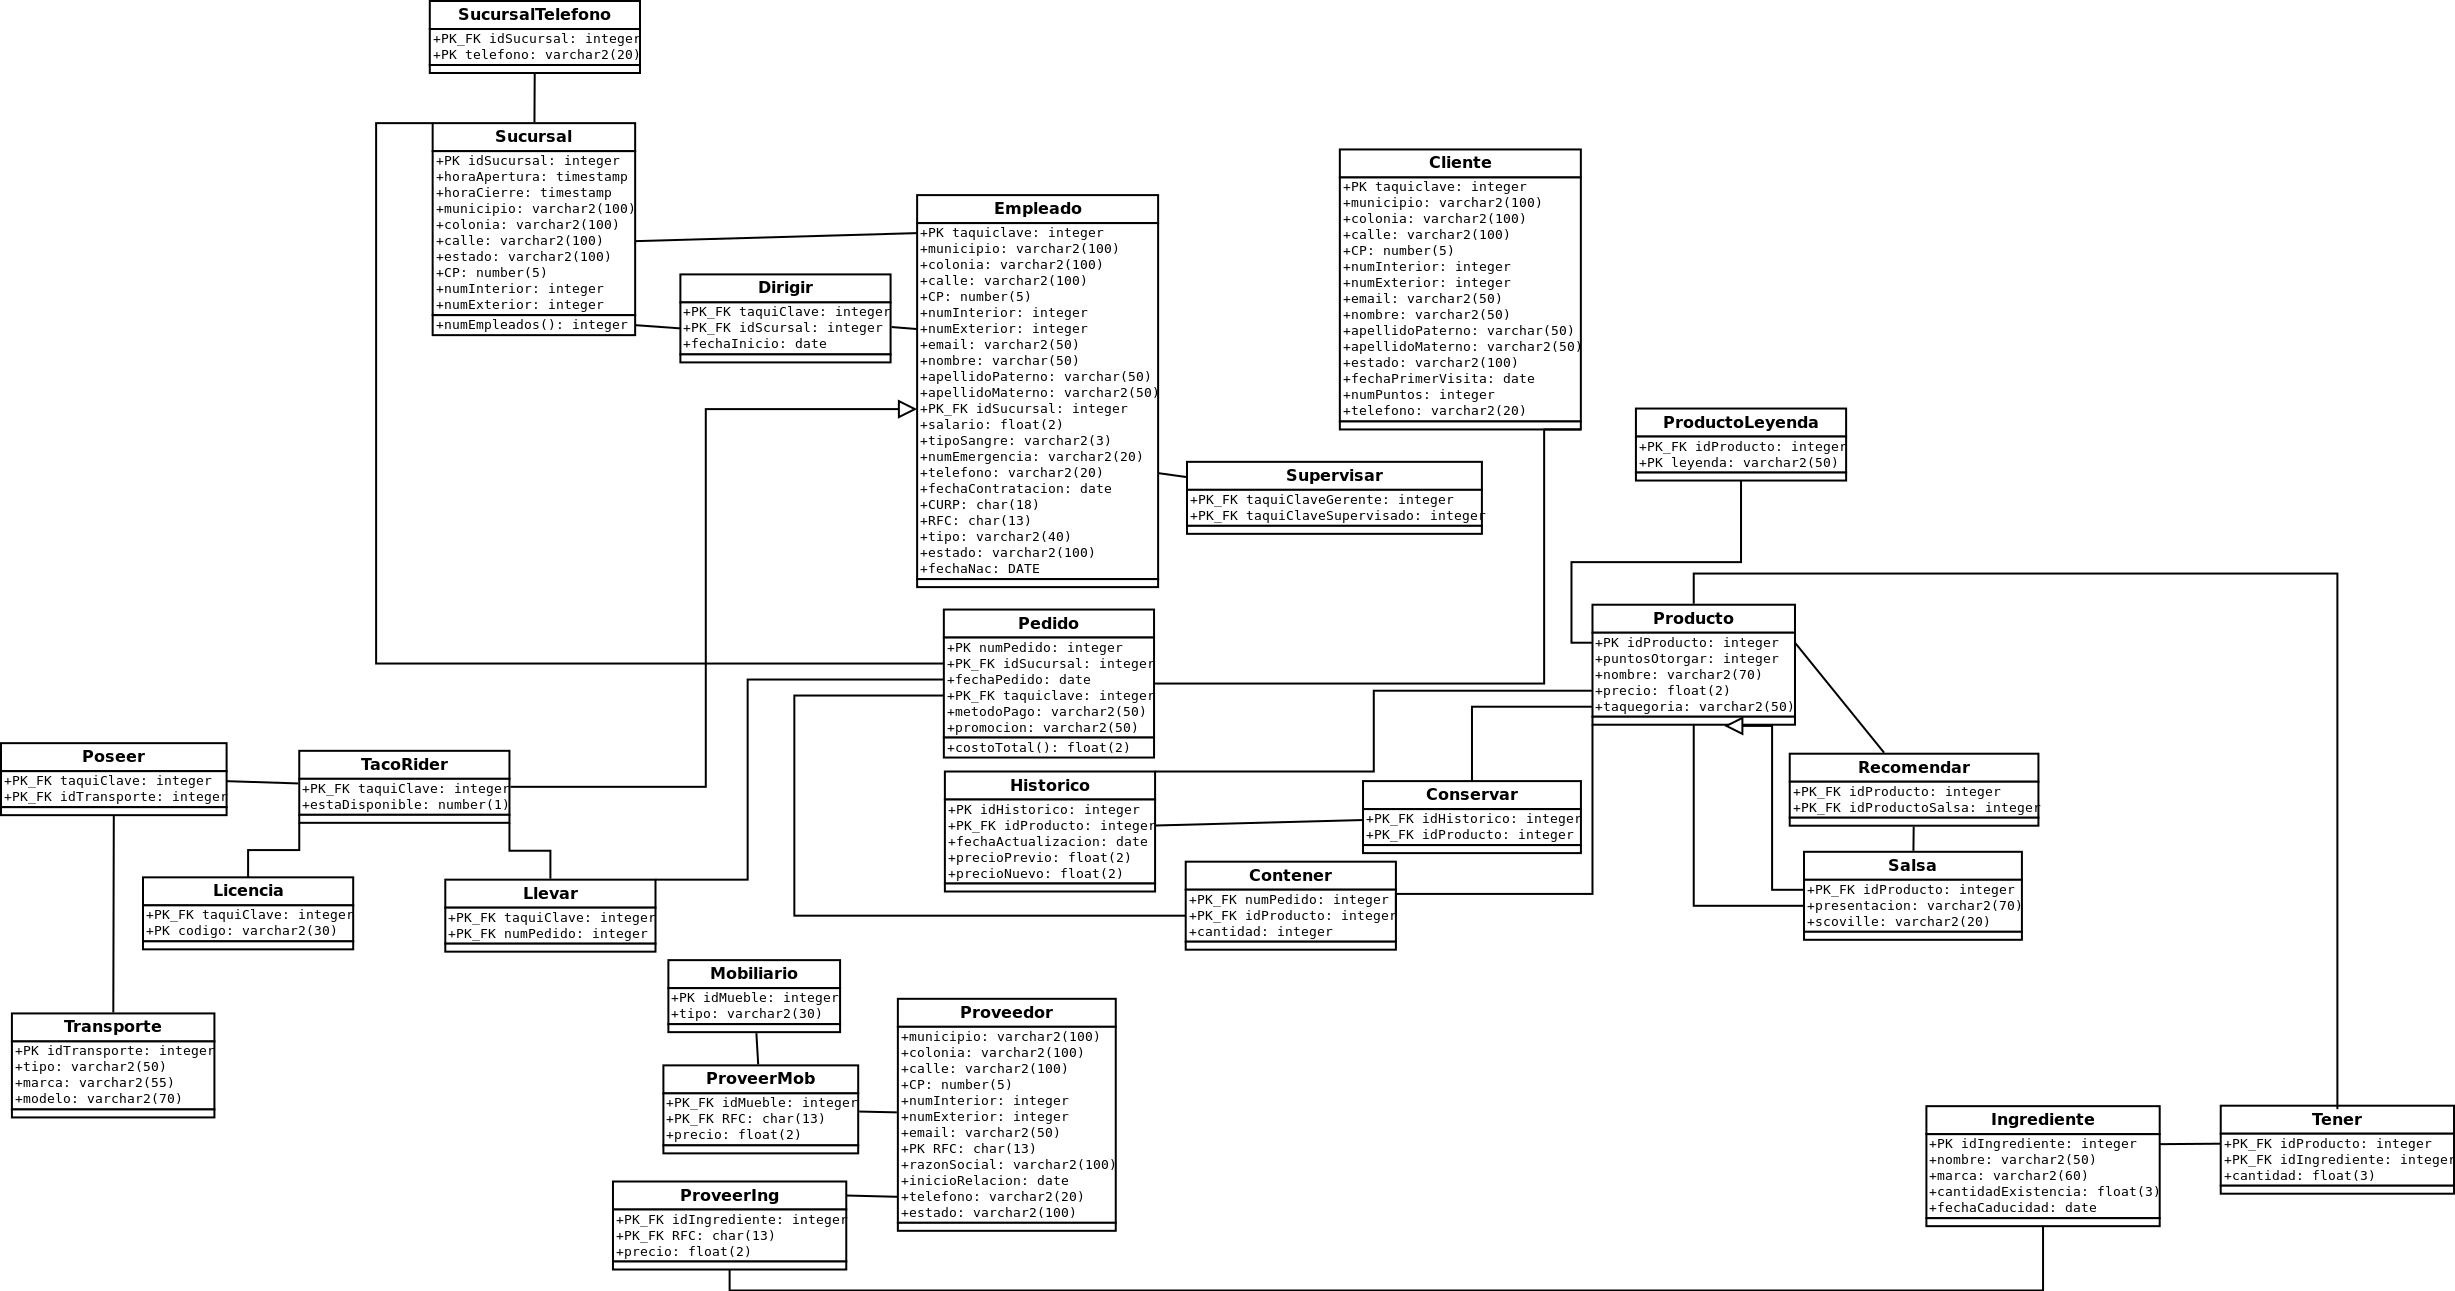
\includegraphics[width=\linewidth]{2NF.png}
\captionof{figure}{Modelo en segunda forma normal.}
\end{minipage}
\end{center}
\end{landscape}
\section{Forma Normal Boyce-Codd (BCNF)}

\subsection{Proceso de Normalización}
Como mencionamos en un inicio, vamos a proceder a normalizar directamente a BCNF y veremos que no se pierden dependencias funcionales. Como la 3NF contiene a BCNF ($BCNF\subset 3NF$), se logrará igualmente una normalización a tercera forma normal.\\

Para que una relación (tabla) esté en esta forma normal, entonces debe-
remos verificar que todo determinante sea llave\footnote{Los determinantes son la parte a la izquierda de las dependencias funcionales, mientras que lo que está la derecha se conoce como determinado.}. En otras palabras y de acuerdo a lo visto con el profesor en clase
tenemos que una relación $R$ está en $BCNF$ si y sólo si en toda DF no trivial $A_1,A_2,\dots, A_n \rightarrow B$ para $R$ se tiene que $\{A_1,A_2,\dots, A_n\}$ es una superllave para $R$. La estrategia para normalizar es:

\begin{enumerate}
\item Buscar una DF no trivial $X\rightarrow B$ que viole BCNF.
\item Calcular la cerradura $X+$.
\item Fraccionar $R$ en $R_1(X+)\cup R_2((R\setminus X+)\cup X)$.
\item Encontrar las DF para las nuevas relaciones.
\end{enumerate}

Normalicemos a partir de esto las tablas cuando sea necesario, considerando las DFs no triviales que pueden, potencialmente, violar la forma normal\footnote{Separaremos con comas (,) los determinados y determinantes para tener mayor claridad, aunque no son necesarias y bien pudimos usar espacios como en la normalización a segunda forma normal.}.

\begin{itemize}

\item \textbf{Categoría}:
\begin{itemize}
\item idProducto $\rightarrow$ taquegoría. Como tenemos que $idProducto^+=\{idProducto,taquegoria\}$, entonces el lado izquierdo es superllave y no hay violación a la forma normal. \checkmark
\end{itemize}

Entonces ya estaba en \textit{BCNF}.


\item \textbf{Cliente}:  Tenemos las DFs:

\begin{itemize}
\item taquiClave $\rightarrow$ email, telefono, nombre, apellidoPaterno, apellidoMaterno,  municipio, colonia, calle, CP, numeroInterior, numExterior, estado, fechaPrimerVisita, numPuntos. \\\\Entonces ocurre que $taquiClave^+ = \{taquiClave,email, telefono, nombre,\\ apellidoPaterno, apellidoMaterno,municipio, colonia, calle, CP, numeroInterior,\\ numExterior, estado, fechaPrimerVisita, numPuntos\}$, así que es superllave y no hay violación \checkmark
\item CP $\rightarrow$ estado. \\\\

Entonces ocurre que $CP^+ = \{CP,estado\}$. Hay violación ya que no cumple con alcanzar el resto de los atributos y por ende no es superllave. \ding{55}
\end{itemize}

Tomando la violación, fraccionamos entonces en dos relaciones, ambas con el determinante de la DF que fue violación, la primera con los atributos determinados de la DF violación y la segunda con los que restan de la relación original. Nos queda así:

\begin{itemize}
\item {\footnotesize \textbf{CPEdoCliente}(\underline{CP},estado)} con:
\begin{itemize}
\item CP $\rightarrow$ estado.\\\\ Tenemos que $CP^+ = \{CP,estado\}$. Entonces, el lado izquierdo es superllave y ya no hay violación \checkmark
\end{itemize}
\item {\footnotesize \textbf{Cliente}(\underline{taquiClave}, email, telefono, nombre, apellidoPaterno, apellidoMaterno,  municipio, colonia, calle, CP, numeroInterior, numExterior, estado, fechaPrimerVisita, numPuntos)} con:
\begin{itemize}
\item taquiClave $\rightarrow$  email, telefono, nombre, apellidoPaterno, apellidoMaterno,  municipio, colonia, calle, CP, numeroInterior, numExterior, estado, fechaPrimerVisita, numPuntos\\\\Como ocurre que $taquiClave^+=\{taquiClave,email, telefono, nombre,\\apellidoPaterno, apellidoMaterno,  municipio, colonia,\\calle, CP, numeroInterior, numExterior, estado, fechaPrimerVisita, numPuntos\}$, entonces el lado izquierdo es superllave y no hay violación. \checkmark
\end{itemize}
\end{itemize}

Y ya hemos normalizado la relación a BCNF.

\item \textbf{Conservar}: La única DF que tenemos es la trivial:

\begin{itemize}
\item idProducto,idHistorico $\rightarrow$ idProducto,idHistorico
\end{itemize}

Entonces, por ser trivial no es candidata a ser violación y ya está en BCNF. En efecto, tenemos que $idProducto,idHistorico^+ = \{idProducto,idHistorico\}$, así que el lado izquierdo es superllave. \checkmark
\item \textbf{Contener}: Tenemos las DFs no triviales siguientes:

\begin{itemize}
\item numPedido,idProducto $\rightarrow$ cantidad.\\ En este caso ocurre que $numPedido,idProducto^+=\{numPedido,idProducto,cantidad\}$, por lo que se cumple que el lado izquierdo es superllave y la relación estaba ya entonces en BCNF. \checkmark
\end{itemize}
\item \textbf{Dirigir}: Tenemos las DFs no triviales siguientes:

\begin{itemize}
\item idSucursal,taquiClave $\rightarrow$ fechaInicio.\\ En este caso ocurre que $idSucursal,taquiClave^+=\{idSucursal,taquiClave,fechaInicio\}$, por lo que se cumple que el lado izquierdo es superllave y la relación estaba ya entonces en BCNF. \checkmark
\end{itemize}
\item \textbf{Empleado}:   Tenemos las DFs:

\begin{itemize}
\item taquiClave $\rightarrow$  idSucursal, salario, email, telefono, nombre, apellidoPaterno, apellidoMaterno,  municipio, colonia, calle, CP, numeroInterior, numExterior, estado, CURP, tipoSangre, numEmergencia, fechaNac, tipo, RFC, fechaContratacion. \\\\Entonces ocurre que $taquiClave^+ = \{idSucursal, salario, email, telefono, nombre,\\ apellidoPaterno, apellidoMaterno,  municipio, colonia, calle,\\CP, numeroInterior, numExterior, estado,\\ CURP, tipoSangre, numEmergencia, fechaNac, tipo, RFC, fechaContratacion\}$, así que es superllave y no hay violación \checkmark
\item CP $\rightarrow$ estado. \\\\

Entonces ocurre que $CP^+ = \{CP,estado\}$. Hay violación ya que no cumple con alcanzar el resto de los atributos y por ende no es superllave. \ding{55}
\item CURP $\rightarrow$ fechaNac.\\\\

Entonces ocurre que $CURP^+ = \{CURP,fechaNac\}$. Hay violación ya que no cumple con alcanzar el resto de los atributos y por ende no es superllave. \ding{55}
\end{itemize}

Tomando la primer violación, fraccionamos entonces en dos relaciones, ambas con el determinante de la DF que fue violación, la primera con los atributos determinados de la DF violación y la segunda con los que restan de la relación original. Nos queda así:

\begin{itemize}
\item {\footnotesize \textbf{CPEdoEmpleado}(\underline{CP},estado)} con:
\begin{itemize}
\item CP $\rightarrow$ estado.\\\\ Tenemos que $CP^+ = \{CP,estado\}$. Entonces, el lado izquierdo es superllave y ya no hay violación \checkmark
\end{itemize}
\item {\footnotesize \textbf{Empleado}(\underline{taquiClave}, idSucursal, salario, email, telefono, nombre, apellidoPaterno, apellidoMaterno,  municipio, colonia, calle, CP, numeroInterior, numExterior, CURP, tipoSangre, numEmergencia, fechaNac, tipo, RFC, fechaContratacion} con:
\begin{itemize}
\item taquiClave $\rightarrow$ idSucursal, salario, email, telefono, nombre, apellidoPaterno, apellidoMaterno,  municipio, colonia, calle, CP, numeroInterior, numExterior,  CURP, tipoSangre, numEmergencia, fechaNac, tipo, RFC, fechaContratacion\\\\Como ocurre que $taquiClave^+=\{taquiClave,idSucursal, salario, email, telefono,\\ nombre, apellidoPaterno, apellidoMaterno,  municipio, colonia, calle,\\ CP, numeroInterior, numExterior,  CURP, tipoSangre,\\ numEmergencia, fechaNac, tipo, RFC, fechaContratacion\}$, entonces el lado izquierdo es superllave; no hay violación. \checkmark
\item CURP $\rightarrow$ fechaNac.\\\\Como $CURP^+ = \{CURP,fechaNac\}$, entonces el lado izquierdo no es superllave y constutya una violación esta DF. \ding{55}
\end{itemize}

Ocupando la DF que fue violación, volvemos a fraccionar:

\begin{itemize}
\item \textbf{CURPFnacEmp}(\underline{CURP}, fechaNac) con CURP $\rightarrow$ fechaNac.\\\\Como ocurre que $CURP^+ = \{CURP,fechaNc\}$, entonces el lado izquierdo es superllave y ya no hay violación. \checkmark
\item {\footnotesize \textbf{Empleado}(\underline{taquiClave}, idSucursal, salario, email, telefono, nombre, apellidoPaterno, apellidoMaterno,  municipio, colonia, calle, CP, numeroInterior, numExterior, CURP, tipoSangre, numEmergencia, fechaNac, tipo, RFC, fechaContratacion} con:
\begin{itemize}
\item taquiClave $\rightarrow$ idSucursal, salario, email, telefono, nombre, apellidoPaterno, apellidoMaterno,  municipio, colonia, calle, CP, numeroInterior, numExterior,  CURP, tipoSangre, numEmergencia, tipo, RFC, fechaContratacion\\\\Como ocurre que $taquiClave^+=\{taquiClave,idSucursal, salario, email,\\ telefono, nombre, apellidoPaterno, apellidoMaterno,  municipio, colonia, calle,\\ CP, numeroInterior, numExterior,  CURP, tipoSangre,\\ numEmergencia, tipo, RFC, fechaContratacion\}$, entonces el lado izquierdo es superllave; no hay violación. \checkmark

\end{itemize}
\end{itemize}
\end{itemize}
Y ya hemos normalizado la relación a BCNF.

\item \textbf{Histórico}: Tenemos las DFs:

\begin{itemize}
\item idHistorico $\rightarrow$ idProducto, fechaActualizacion, precioPrevio, precioNuevo. \\\\Entonces ocurre que $idHistorico^+ = \{idProducto, fechaActualizacion, \\precioPrevio, precioNuevo\}$, así que es superllave y no hay violación \checkmark
\end{itemize}
Entonces la relación estaba ya en BCNF.
\item \textbf{Ingrediente}: Contamos con las DFs no triviales:

\begin{itemize}
\item idIngrediente $\rightarrow$ nombre, marca, cantidadExistencia, fechaCaducidad.\\Se tiene que $idIngrediente^+=\{idIngrediente,nombre, marca,\\cantidadExistencia, fechaCaducidad\}$, así que el lado izquierdo es superllave y no es violación a la forma normal. \checkmark
\item nombre  $\rightarrow$  idIngrediente, marca, cantidadExistencia, fechaCaducidad.\\Se tiene que $nombre^+=\{nombre,idIngrediente, marca, \\cantidadExistencia, fechaCaducidad\}$, así que el lado izquierdo es superllave y no es violación a la forma normal. \checkmark
\end{itemize}

Entonces ya estaba en BCNF.
\item \textbf{Licencia}: La única DF no trivial con que se cuenta es:
\begin{itemize}
\item codigo $\rightarrow$ taquiClave. Como tenemos que $codigo^+ = \{codigo,taquiClave\}$, se tiene que el lado izquierdo es superllave y no constituye una violación a BCNF. \checkmark
\end{itemize}
\item \textbf{Llevar}: La única DF que tenemos es la trivial:

\begin{itemize}
\item taquiClave,numPedido $\rightarrow$ taquiClave,numPedido
\end{itemize}

Entonces, por ser trivial no es candidata a ser violación y ya está en BCNF. En efecto, tenemos que $taquiClave,numPedido^+ = \{taquiClave,numPedido\}$, así que el lado izquierdo es superllave. \checkmark
\item \textbf{Mobiliario}: La única DF no trivial con que se cuenta es:
\begin{itemize}
\item idMueble $\rightarrow$ tipo. Como tenemos que $idMueble^+ = \{idMueble,tipo\}$, se tiene que el lado izquierdo es superllave y no constituye una violación a BCNF. \checkmark
\end{itemize}
\item \textbf{Pedido}: Tenemos las DFs:

\begin{itemize}
\item numPedido $\rightarrow$ idSucursal, fechaPedido, taquiClave, metodoPago, promocion,preparado,entregado. \\\\Entonces ocurre que $numPedido^+ = \{numPedido,idSucursal, fechaPedido, taquiClave,\\ metodoPago, promocion,preparado,entregado\}$, así que es superllave y no hay violación \checkmark
\item fechaPedido $\rightarrow$ promocion. \\\\

Entonces ocurre que $fechaPedido^+ = \{fechaPedido,promocion\}$. Hay violación ya que no cumple con alcanzar el resto de los atributos y por ende no es superllave. \ding{55}
\end{itemize}

Tomando la violación, fraccionamos entonces en dos relaciones, ambas con el determinante de la DF que fue violación, la primera con los atributos determinados de la DF violación y la segunda con los que restan de la relación original. Nos queda así:

\begin{itemize}
\item {\footnotesize \textbf{fechaPedPromo}(\underline{fechaPedido},promocion)} con:
\begin{itemize}
\item fechaPedido $\rightarrow$ promocion.\\\\ Tenemos que $fechaPedido^+ = \{fechaPedido,promocion\}$. Entonces, el lado izquierdo es superllave y ya no hay violación \checkmark
\end{itemize}
\item {\footnotesize \textbf{Pedido}(\underline{numPedido}, idSucursal, fechaPedido, taquiClave, metodoPago,preparado,entregado}) con:
\begin{itemize}
\item numPedido $\rightarrow$ idSucursal, fechaPedido, taquiClave, metodoPago,entregado,preparado\\\\Como ocurre que $numPedido^+=\{idSucursal, fechaPedido, taquiClave, metodoPago,\\preparado,entregado\}$, entonces el lado izquierdo es superllave y no hay violación. \checkmark
\end{itemize}
\end{itemize}

Y ya hemos normalizado la relación a BCNF.
\item \textbf{Poseer}: La única DF que tenemos es la trivial:

\begin{itemize}
\item taquiClave,idTransporte $\rightarrow$ taquiClave,idTransporte
\end{itemize}

Entonces, por ser trivial no es candidata a ser violación y ya está en BCNF. En efecto, tenemos que $taquiClave,idTransporte^+ = \{taquiClave,idTransporte\}$, así que el lado izquierdo es superllave. \checkmark
\item \textbf{Producto}: Contamos con las DFs no triviales:

\begin{itemize}
\item idProducto $\rightarrow$ nombre, precio, descripcion.\\Se tiene que $idProducto^+=\{idProducto, nombre, precio, descripcion\}$, así que el lado izquierdo es superllave y no es violación a la forma normal. \checkmark
\item nombre $\rightarrow$ idProducto, precio, descripcion.\\Se tiene que $nombre^+=\{nombre, idProducto, precio, descripcion\}$, así que el lado izquierdo es superllave y no es violación a la forma normal. \checkmark
\end{itemize}

Entonces ya estaba en BCNF.
\item \textbf{ProductoLeyenda}: La única DF es la trivial es:

\begin{itemize}
\item idProducto,leyenda $\rightarrow$ idProducto leyenda. Al ser trivial, entonces no es candidata a ser violación. EN efecto, tenemos que $ idProducto,leyenda^+=\{idProducto,leyenda\}$, por lo que el lado izquierdo es superllave. Está ya en BCNF. \checkmark
\end{itemize}
\item \textbf{Proveedor}:  Tenemos las DFs:

\begin{itemize}
\item RFC $\rightarrow$  razonSocial, inicioRelacion, email, telefono,  municipio, colonia, calle, CP, numeroInterior, numExterior, estado. \\\\Entonces ocurre que $RFC^+ = \{razonSocial, inicioRelacion, email,\\ telefono,  municipio, colonia, calle, \\CP, numeroInterior, numExterior, estado\}$, así que es superllave y no hay violación \checkmark
\item CP $\rightarrow$ estado. \\\\

Entonces ocurre que $CP^+ = \{CP,estado\}$. Hay violación ya que no cumple con alcanzar el resto de los atributos y por ende no es superllave. \ding{55}
\end{itemize}

Tomando la violación, fraccionamos entonces en dos relaciones, ambas con el determinante de la DF que fue violación, la primera con los atributos determinados de la DF violación y la segunda con los que restan de la relación original. Nos queda así:

\begin{itemize}
\item {\footnotesize \textbf{CPEdoProveedor}(\underline{CP},estado)} con:
\begin{itemize}
\item CP $\rightarrow$ estado.\\\\ Tenemos que $CP^+ = \{CP,estado\}$. Entonces, el lado izquierdo es superllave y ya no hay violación \checkmark
\end{itemize}
\item {\footnotesize \textbf{Proveedor}(\underline{RFC}, razonSocial, inicioRelacion, email, telefono,  municipio, colonia, calle, CP, numeroInterior, numExterior, estado} con:
\begin{itemize}
\item RFC $\rightarrow$  razonSocial, inicioRelacion, email, telefono,  municipio, colonia, calle, CP, numeroInterior, numExterior\\\\Como ocurre que $RFC^+=\{RFC,razonSocial, inicioRelacion, email,\\telefono,  municipio, colonia, calle,\\ CP, numeroInterior, numExterior\}$, entonces el lado izquierdo es superllave y no hay violación. \checkmark
\end{itemize}
\end{itemize}

Y ya hemos normalizado la relación a BCNF.

\item \textbf{ProveerIng}: La única DF no trivial es:

\begin{itemize}
\item RFC,idIngrediente $\rightarrow$ precio.\\Ocurre que ya está en BCNF porque el lado izquierdo es superllave como vemos por la cerradura $RFC,idIngrediente^+=\{RFC,idIngrediente,precio\}$. \checkmark
\end{itemize}
\item \textbf{ProveerMob}: La única DF no trivial es:

\begin{itemize}
\item RFC,idMueble $\rightarrow$ precio.\\Ocurre que ya está en BCNF porque el lado izquierdo es superllave como vemos por la cerradura $RFC,idMueble^+=\{RFC,idMueble,precio\}$. \checkmark
\end{itemize}
\item \textbf{Recomendar}: La única DF que tenemos es la trivial:

\begin{itemize}
\item idProducto,idProductoSalsa $\rightarrow$ idProducto,idProductoSalsa
\end{itemize}

Entonces, por ser trivial no es candidata a ser violación y ya está en BCNF. En efecto, tenemos que $idProducto,idProductoSalsa^+ = \{idProducto,idProductoSalsa\}$, así que el lado izquierdo es superllave. \checkmark

\item \textbf{Salsa}: Contamos con las DFs no triviales:

\begin{itemize}
\item idProducto $\rightarrow$ nombre, presentacion, scoville.\\Se tiene que $idProducto^+=\{idProducto,nombre, presentacion, scoville\}$, así que el lado izquierdo es superllave y no es violación a la forma normal. \checkmark
\item nombre $\rightarrow$ idProducto, presentacion, scoville.\\Se tiene que $nombre^+=\{nombre,idProducto, presentacion, scoville\}$, así que el lado izquierdo es superllave y no es violación a la forma normal. \checkmark
\end{itemize}

Entonces ya estaba en BCNF.
\item \textbf{Sucursal}:   Tenemos las DFs:

\begin{itemize}
\item idSucursal $\rightarrow$ horaApertura, horaCierre, municipio, colonia, calle, CP, numInterior, numExterior, estado. \\\\Entonces ocurre que $idSucursal^+ = \{idSucursal,horaApertura, horaCierre, municipio,\\colonia, calle, CP, numInterior, numExterior, estado\}$, así que es superllave y no hay violación \checkmark
\item CP $\rightarrow$ estado. \\\\

Entonces ocurre que $CP^+ = \{CP,estado\}$. Hay violación ya que no cumple con alcanzar el resto de los atributos y por ende no es superllave. \ding{55}
\end{itemize}

Tomando la violación, fraccionamos entonces en dos relaciones, ambas con el determinante de la DF que fue violación, la primera con los atributos determinados de la DF violación y la segunda con los que restan de la relación original. Nos queda así:

\begin{itemize}
\item {\footnotesize \textbf{CPEdoSucursal}(\underline{CP},estado)} con:
\begin{itemize}
\item CP $\rightarrow$ estado.\\\\ Tenemos que $CP^+ = \{CP,estado\}$. Entonces, el lado izquierdo es superllave y ya no hay violación \checkmark
\end{itemize}
\item {\footnotesize \textbf{Sucursal}(CP,\underline{idSucursal}, horaApertura, horaCierre, municipio, colonia, calle, numInterior, numExterior)} con:
\begin{itemize}
\item idSucursal $\rightarrow$ horaApertura, horaCierre, municipio, colonia, calle, CP, numInterior, numExterior\\\\Como ocurre que $idSucursal^+=\{idSucursal,horaApertura, horaCierre, municipio,\\ colonia, calle, CP, numInterior, numExterior\}$, entonces el lado izquierdo es superllave y no hay violación. \checkmark
\end{itemize}
\end{itemize}

Y ya hemos normalizado la relación a BCNF.

\item \textbf{SucursalTelefono}: La única DF no trivial es:

\begin{itemize}
\item telefono $\rightarrow$ idSucursal.\\Ocurre que $telefono^+=\{telefono,idSucursal\}$. Como el lado izquierdo es una superllave de la relación, entonces se cumple con que no hay una violación a la forma normal y en consecuencia estaba ya en BCNF. \checkmark
\end{itemize}
\item \textbf{Supervisar}: La única DF que tenemos es la trivial:

\begin{itemize}
\item taquiClaveGerente,taquiClaveSupervisado $\rightarrow$ taquiClaveGerente,taquiClaveSupervisado
\end{itemize}

Entonces, por ser trivial no es candidata a ser violación y ya está en BCNF. En efecto, tenemos que $taquiClaveGerente,taquiClaveSupervisado^+ = \{taquiClaveGerente,taquiClaveSupervisado\}$, así que el lado izquierdo es superllave. \checkmark
\item \textbf{TacoRider}: La única DF con que se cuenta es:

\begin{itemize}
\item taquiClave $\rightarrow$ estaDisponible.\\ Tenemos que $taquiClave^+=\{taquiClave,estaDisponible\}$, por lo que el lado izquierdo es superllave y no constituye una violación a la forma normal. Estaba ya en BCNF. \checkmark
\end{itemize}
\item \textbf{Tener}: La única DF con que se cuenta es:

\begin{itemize}
\item idProducto, idIngrediente $\rightarrow$  cantidad.\\ Tenemos que $idProducto, idIngrediente^+=\{idProducto, idIngrediente,cantidad\}$, por lo que el lado izquierdo es superllave y no constituye una violación a la forma normal. Estaba ya en BCNF. \checkmark
\end{itemize}
\item \textbf{Transporte}: Las DFs no triviales son:

\begin{itemize}
\item idTransporte $\rightarrow$  tipo, marca, modelo.\\Como la cerradura es $idTransporte^+ =\{idTransporte,tipo, marca, modelo\}$, se cumple que el lado izquierdo es superllave y estaba ya en BCNF entonces. \checkmark
\end{itemize}
\end{itemize}

\subsection{Relaciones Generadas}
Entonces, en resumidas cuentas contamos con las siguientes relaciones luego de la normalización a BCNF obtenemos:

\begin{itemize}
\item \footnotesize{\textbf{Categoría}(\underline{idProducto},taquegoria)}
\item \footnotesize{\textbf{Cliente}(\underline{taquiClave},email,telefono,nombre,apellidoPaterno,apellidoMaterno,calle,municipio,colonia,
numInterior,numExterior,CP,numPuntos,fechaPrimerVisita)}
\item \footnotesize{\textbf{Conservar}(\underline{idHistorico},\underline{idProducto})}
\item \footnotesize{\textbf{Contener}(\underline{numPedido},\underline{idProducto},cantidad)}
\item {\footnotesize \textbf{CPEdoCliente}(\underline{CP}, estado)}
\item {\footnotesize \textbf{CPEdoEmpleado}(\underline{CP}, estado)} 
\item {\footnotesize \textbf{CPEdoProveedor}(\underline{CP}, estado) }
\item {\footnotesize \textbf{CPEdoSurcursal}(\underline{CP}, estado)}
\item{\footnotesize  \textbf{CURPFnacEmp}(\underline{CURP}, fechaNac) }
\item{\footnotesize  \textbf{FechaPedPromo}(\underline{fechaPedido}, promocion) }
\item \footnotesize{\textbf{Dirigir}(\underline{taquiClave},\underline{idSucursal},fechaInicio)}
\item \footnotesize{\textbf{Empleado}(\underline{taquiClave},email,telefono,nombre,apellidoPaterno,apellidoMaterno,calle,municipio,colonia,
numInterior,numExterior,CP,CURP,RFC,tipo,tipoSangre,fechaContratacion,
numEmergencia,salario,\underline{idSucursal})}
\item \footnotesize{\textbf{Historico}(\underline{idHistorico},idProducto,precioPrevio,precioNuevo,fechaActualizacion)}
\item \footnotesize{\textbf{Ingrediente}(\underline{idIngrediente},nombre,marca,cantidadExistencia,fechaCaducidad)}
\item \footnotesize{\textbf{Licencia}(\underline{codigo},\underline{taquiClave}})
\item \footnotesize{\textbf{Llevar}(\underline{numPedido},\underline{taquiClave})}
\item \footnotesize{\textbf{Mobiliario}(\underline{idMueble},tipo)}
\item \footnotesize{\textbf{Pedido}(\underline{numPedido},fechaPedido,\underline{taquiClave},metodoPago,\underline{idSucursal},preparado,entregado)}
\item \footnotesize{\textbf{Poseer}(\underline{taquiClave},\underline{idTransporte})}
\item \footnotesize{\textbf{Producto}(\underline{idProducto},nombre,precio,descripcion)}
\item \footnotesize{\textbf{ProductoLeyenda}(\underline{idProducto,leyenda})}
\item \scriptsize{\textbf{Proveedor}(\underline{RFC},razonSocial,calle,municipio,colonia,numInterior,numExterior,CP,email,inicioRelacion,telefono)}
\item \footnotesize{\textbf{ProveerIng}(\underline{RFC},\underline{idIngrediente},precio)}
\item \footnotesize{\textbf{ProveerMob}(\underline{RFC},\underline{idMueble},precio)}
\item \footnotesize{\textbf{Recomendar}(\underline{idProducto},\underline{idProductoSalsa})}
\item \footnotesize{\textbf{Salsa}(\underline{idProducto},scoville,presentacion)}
\item {\footnotesize \textbf{Sucursal}(\underline{idSucursal},calle,municipio,colonia,numInterior,numExterior,CP,horaApertura,horaCierre)}
\item \footnotesize{\textbf{SucursalTelefono}(\underline{idSucursal},\underline{telefono})}
\item \footnotesize{\textbf{Supervisar}(\underline{taquiClaveGerente},\underline{taquiClaveSupervisado})}
\item \footnotesize{\textbf{TacoRider}(\underline{taquiClave},estaDisponible)}
\item \footnotesize{\textbf{Tener}(\underline{idProducto},\underline{idIngrediente},cantidad)}
\item \footnotesize{\textbf{Transporte}(\underline{idTransporte},marca,modelo,tipo)}

\end{itemize}
\subsection{Diagrama de Clase UML}

 \begin{landscape}
\begin{center}
\begin{minipage}{1\linewidth}
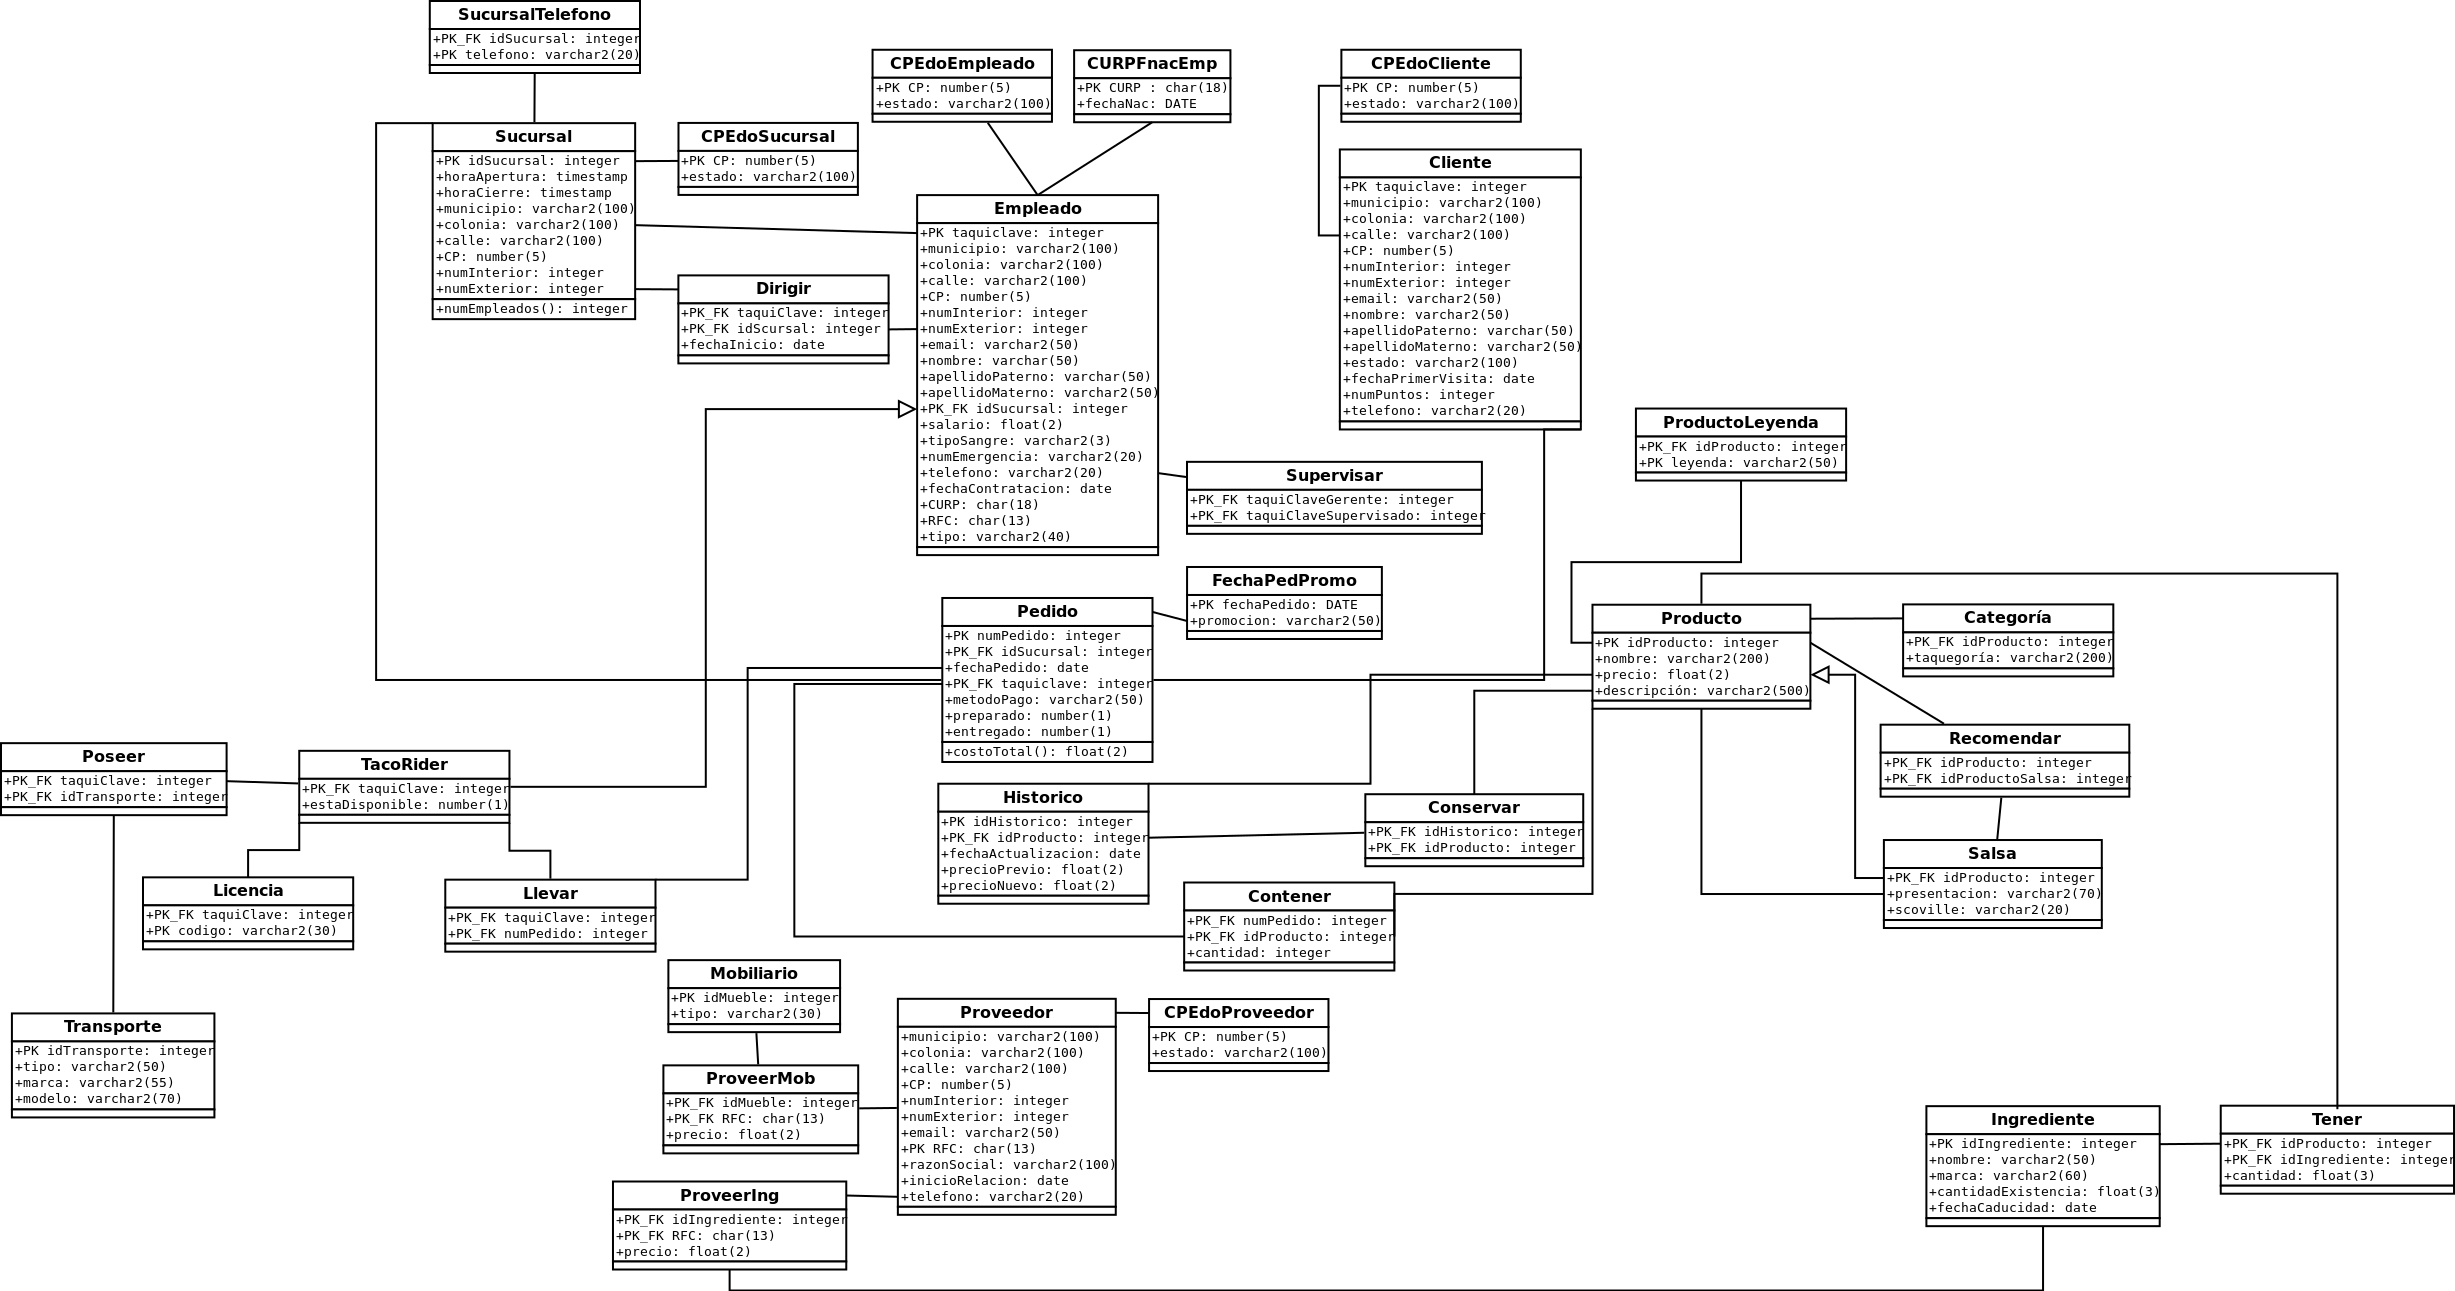
\includegraphics[width=\linewidth]{UML_normalizado.png}
\captionof{figure}{Modelo en forma normal Boyce-Codd.}
\end{minipage}
\end{center}
\end{landscape}
\section{Tercera Forma Normal (3NF)}

\subsection{Proceso de Normalización}
Tomando como base el resultado de la normalización a segunda forma normal ---que de hecho fue igual que nuestro modelo relacional original al no haber sufrido ninguna alteración---, vamos a normalizar a \textit{tercera forma normal} como hubiéramos hecho en caso de haber perdido dependencias funcionales al tratar de llevar a la forma normal más rígida de BCNF, lo cual no fue nuestro caso.\\

Recordemos para este motivo brevemente que una relación $R$ está en 3NF si ocurre que para toda DF no trivial $A_1,A_2,\dots, A_n\rightarrow B$ se tiene que (alguna o ambas):

\begin{itemize}
\item El lado izquierdo ($A_1,A_2,\dots, A_n$) es una superllave.
\item El lado derecho, $B$, es miembro de alguna llave candidata de $R$.
\end{itemize}

Para poder normalizar, debemos seguir el siguiente algoritmo de síntesis revisado a profundidad en el curso:

\begin{enumerate}
\item Hacer $F$ (el conjunto de dependencias funcionales) mínimo.
\item Para toda DF en $F$ mínimo:
\begin{enumerate}
\item Crear una relación que contenga sólo los atributos de las DF.
\item Eliminar un esquema si es subconjunto de otro.
\end{enumerate}
\item Si no existen esquemas que contengan llaves candidatas, crear una relación con esos atributos.
\end{enumerate}

\begin{itemize}
\item \textbf{Categoría}: La única dependencia funcional no trivial es:

\begin{itemize}
\item idProducto $\rightarrow$ taquegoría. Como tenemos que $idProducto^+=\{idProducto,taquegoria\}$, entonces el lado izquierdo es superllave y no hay violación a la forma normal.
\end{itemize}

Entonces ya estaba en \textit{tercera forma normal}.


\item \textbf{Cliente}: Tenemos las dependencias funcionales no triviales que constituyen el conjunto $F$ son las que siguen:

\begin{itemize}
\item taquiClave $\rightarrow$ email, telefono, nombre, apellidoPaterno, apellidoMaterno,  municipio, colonia, calle, CP, numeroInterior, numExterior, estado, fechaPrimerVisita, numPuntos. No viola la forma normal porque el atributo \textit{taquiClave} es una superllave ya que la cerradura permite alcanzar todos los atributos de la relación. 
\item CP $\rightarrow$ estado. Viola la forma normal porque el lado derecho, no forma parte de una llave candidata. Esto se debe a que $estado^+ =\{estado\}$ y para ser llave candidata debería alcanzar a todos los atributos porque a partir del punto previo vimos que a partir de un solo atributo, \textit{taquiClave}, sí se pueden alcanzar todos.
\end{itemize}



Entonces busquemos primero $F$ mínimo. Potencialmente puede haber atributos superfluos por la derecha de la primera DF. VEamos si los hay:

\begin{itemize}
\item ¿\textit{email} es superfluo por la derecha? Tenemos en este caso $F'=\{taquiClave \rightarrow telefono, nombre, apellidoPaterno, apellidoMaterno,  municipio,\\colonia, calle, CP, numeroInterior, numExterior, estado,\\fechaPrimerVisita, numPuntos, CP\rightarrow estado\}$. Si obtenemos la cerradura $taquiClave^+=\{taquiClave,telefono, nombre, apellidoPaterno,\\ apellidoMaterno,  municipio,\\colonia, calle, CP, numeroInterior, numExterior, estado,\\fechaPrimerVisita, numPuntos\}$, pero no tiene a \textit{email} como elemento, así que no es superfluo por la derecha.
\item ¿\textit{telefono} es superfluo por la derecha? Tenemos en este caso $F'=\{taquiClave \rightarrow email, nombre, apellidoPaterno, apellidoMaterno,  municipio,\\colonia, calle, CP, numeroInterior, numExterior, estado,\\fechaPrimerVisita, numPuntos, CP\rightarrow estado\}$. Si obtenemos la cerradura $taquiClave^+=\{taquiClave,email, nombre, apellidoPaterno,\\ apellidoMaterno,  municipio,\\colonia, calle, CP, numeroInterior, numExterior, estado,\\fechaPrimerVisita, numPuntos\}$, pero no tiene a \textit{telefono} como elemento, así que no es superfluo por la derecha.
\item ¿\textit{nombre} es superfluo por la derecha? Tenemos en este caso $F'=\{taquiClave \rightarrow email, telefono, apellidoPaterno, apellidoMaterno,  municipio,\\colonia, calle, CP, numeroInterior, numExterior, estado,\\fechaPrimerVisita, numPuntos, CP\rightarrow estado\}$. Si obtenemos la cerradura $taquiClave^+=\{taquiClave,email, telefono, apellidoPaterno,\\ apellidoMaterno,  municipio,\\colonia, calle, CP, numeroInterior, numExterior, estado,\\fechaPrimerVisita, numPuntos\}$, pero no tiene a \textit{nombre} como elemento, así que no es superfluo por la derecha.
\item ¿\textit{apellidoPaterno} es superfluo por la derecha? Tenemos en este caso $F'=\{taquiClave \rightarrow email, telefono, nombre, apellidoMaterno,  municipio,\\colonia, calle, CP, numeroInterior, numExterior, estado,\\fechaPrimerVisita, numPuntos, CP\rightarrow estado\}$. Si obtenemos la cerradura $taquiClave^+=\{taquiClave,email, telefono, nombre,\\ apellidoMaterno,  municipio,\\colonia, calle, CP, numeroInterior, numExterior, estado,\\fechaPrimerVisita, numPuntos\}$, pero no tiene a \textit{apellidoPaterno} como elemento, así que no es superfluo por la derecha.
\item ¿\textit{apellidoMaterno} es superfluo por la derecha? Tenemos en este caso $F'=\{taquiClave \rightarrow email, telefono, nombre, apellidoPaterno,  municipio,\\colonia, calle, CP, numeroInterior, numExterior, estado,\\fechaPrimerVisita, numPuntos, CP\rightarrow estado\}$. Si obtenemos la cerradura $taquiClave^+=\{taquiClave,email, telefono, nombre,\\ apellidoPaterno,  municipio,\\colonia, calle, CP, numeroInterior, numExterior, estado,\\fechaPrimerVisita, numPuntos\}$, pero no tiene a \textit{apellidoMaterno} como elemento, así que no es superfluo por la derecha.
\item ¿\textit{municipio} es superfluo por la derecha? Tenemos en este caso $F'=\{taquiClave \rightarrow email, telefono, nombre, apellidoPaterno,  apellidoMaterno,\\colonia, calle, CP, numeroInterior, numExterior, estado,\\fechaPrimerVisita, numPuntos, CP\rightarrow estado\}$. Si obtenemos la cerradura $taquiClave^+=\{taquiClave,email, telefono, nombre,\\ apellidoPaterno,  apellidoMaterno,\\colonia, calle, CP, numeroInterior, numExterior, estado,\\fechaPrimerVisita, numPuntos\}$, pero no tiene a \textit{municipio} como elemento, así que no es superfluo por la derecha.
\item ¿\textit{colonia} es superfluo por la derecha? Tenemos en este caso $F'=\{taquiClave \rightarrow email, telefono, nombre, apellidoPaterno,  apellidoMaterno,\\municipio, calle, CP, numeroInterior, numExterior, estado,\\fechaPrimerVisita, numPuntos, CP\rightarrow estado\}$. Si obtenemos la cerradura $taquiClave^+=\{taquiClave,email, telefono, nombre,\\ apellidoPaterno,  apellidoMaterno,\\municipio, calle, CP, numeroInterior, numExterior, estado,\\fechaPrimerVisita, numPuntos\}$, pero no tiene a \textit{colonia} como elemento, así que no es superfluo por la derecha.
\item ¿\textit{calle} es superfluo por la derecha? Tenemos en este caso $F'=\{taquiClave \rightarrow email, telefono, nombre, apellidoPaterno,  apellidoMaterno,\\municipio, colonia, CP, numeroInterior, numExterior, estado,\\fechaPrimerVisita, numPuntos, CP\rightarrow estado\}$. Si obtenemos la cerradura $taquiClave^+=\{taquiClave,email, telefono, nombre,\\ apellidoPaterno,  apellidoMaterno,\\municipio, colonia, CP, numeroInterior, numExterior, estado,\\fechaPrimerVisita, numPuntos\}$, pero no tiene a \textit{calle} como elemento, así que no es superfluo por la derecha.
\item ¿\textit{CP} es superfluo por la derecha? Tenemos en este caso $F'=\{taquiClave \rightarrow email, telefono, nombre, apellidoPaterno,  apellidoMaterno,\\municipio, colonia, calle, numeroInterior, numExterior, estado,\\fechaPrimerVisita, numPuntos, CP\rightarrow estado\}$. Si obtenemos la cerradura $taquiClave^+=\{taquiClave,email, telefono, nombre,\\ apellidoPaterno,  apellidoMaterno,\\municipio, colonia, calle, numeroInterior, numExterior, estado,\\fechaPrimerVisita, numPuntos\}$, pero no tiene a \textit{CP} como elemento, así que no es superfluo por la derecha.
\item ¿\textit{numInterior} es superfluo por la derecha? Tenemos en este caso $F'=\{taquiClave \rightarrow email, telefono, nombre, apellidoPaterno,  apellidoMaterno,\\municipio, colonia, calle, CP, numExterior, estado,\\fechaPrimerVisita, numPuntos, CP\rightarrow estado\}$. Si obtenemos la cerradura $taquiClave^+=\{taquiClave,email, telefono, nombre,\\ apellidoPaterno,  apellidoMaterno,\\municipio, colonia, calle, CP, numExterior, estado,\\fechaPrimerVisita, numPuntos\}$, pero no tiene a \textit{numInterior} como elemento, así que no es superfluo por la derecha.
\item ¿\textit{numExterior} es superfluo por la derecha? Tenemos en este caso $F'=\{taquiClave \rightarrow email, telefono, nombre, apellidoPaterno,  apellidoMaterno,\\municipio, colonia, calle, CP, numInterior, estado,\\fechaPrimerVisita, numPuntos, CP\rightarrow estado\}$. Si obtenemos la cerradura $taquiClave^+=\{taquiClave,email, telefono, nombre,\\ apellidoPaterno,  apellidoMaterno,\\municipio, colonia, calle, CP, numInterior, estado,\\fechaPrimerVisita, numPuntos\}$, pero no tiene a \textit{numExterior} como elemento, así que no es superfluo por la derecha.
\item ¿\textit{fechaPrimerVisita} es superfluo por la derecha? Tenemos en este caso $F'=\{taquiClave \rightarrow email, telefono, nombre, apellidoPaterno,  apellidoMaterno,\\municipio, colonia, calle, CP, numInterior, numExterior, estado,\\, numPuntos, CP\rightarrow estado\}$. Si obtenemos la cerradura $taquiClave^+=\{taquiClave,email, telefono, nombre,\\ apellidoPaterno,  apellidoMaterno,\\municipio, colonia, calle, CP, numInterior,numExterior, estado,\\, numPuntos\}$, pero no tiene a \textit{fechaPrimerVisita} como elemento, así que no es superfluo por la derecha.
\item ¿\textit{numPuntos} es superfluo por la derecha? Tenemos en este caso $F'=\{taquiClave \rightarrow email, telefono, nombre, apellidoPaterno,  apellidoMaterno,\\municipio, colonia, calle, CP, numInterior, numExterior, estado,\\, fechaPrimerVisita, CP\rightarrow estado\}$. Si obtenemos la cerradura $taquiClave^+=\{taquiClave,email, telefono, nombre,\\ apellidoPaterno,  apellidoMaterno,\\municipio, colonia, calle, CP, numInterior,numExterior, estado,\\, fechaPrimerVisita\}$, pero no tiene a \textit{numPuntos} como elemento, así que no es superfluo por la derecha.
\item ¿\textit{estado} es superfluo por la derecha? Tenemos en este caso $F'=\{taquiClave \rightarrow email, telefono, nombre, apellidoPaterno,  apellidoMaterno,\\municipio, colonia, calle, CP, numInterior, numExterior,\\, fechaPrimerVisita, CP\rightarrow estado\}$. Si obtenemos la cerradura $taquiClave^+=\{taquiClave,email, telefono, nombre,\\ apellidoPaterno,  apellidoMaterno,\\municipio, colonia, calle, CP, numInterior,numExterior, estado,\\, fechaPrimerVisita\}$, y veamos que en este caso tiene a \textit{estado} como elemento, así que \textbf{sí} es superfluo por la derecha.
\end{itemize}

Por tanto, el conjunto $F$ mínimo (cada lado izquierdo de las DFs es único y ya no hay atributos superfluos) tiene como DFs:

\begin{itemize}
\item taquiClave $\rightarrow$ email, telefono, nombre, apellidoPaterno, apellidoMaterno,  municipio, colonia, calle, CP, numeroInterior, numExterior, fechaPrimerVisita, numPuntos
\item CP $\rightarrow$ estado
\end{itemize}

Entonces procedemos a crear relaciones para cada DF con los atributos que aparezcan en ésta. Obtenemos:

\begin{itemize}
\item {\footnotesize \textbf{Cliente}(\underline{taquiClave},email, telefono, nombre, apellidoPaterno, apellidoMaterno,  municipio, colonia, calle, CP, numeroInterior, numExterior, fechaPrimerVisita, numPuntos)}
\item {\footnotesize \textbf{CPEdoCliente(\underline{CP},estado)}}
\end{itemize}

El primer esquema contiene a la llave candidata \textit{taquiClave}, así que no debemos añadir nuevas relaciones. Además, ningún esquema es subconjunto de otro. Hemos normalizado a \textit{tercera forma normal} la relación. \\

A partir de este punto especificaremos directamente cuando existan atributos que sean superfluos por la izquierda o derecha y verificaremos que en efecto lo son; para aquellos que no lo sean, dejamos el proceso de revisión al lector ya que son análogos al que se hizo en este caso y es fácil ver que no lo serán ya que en casi todos los casos de nuestro modelo ocurrirán casos muy similares puesto que las llaves candidatas son las llaves primarias de la relación conformadas por ---casi siempre--- un único atributo. 
%%%%%%%%%%%%%%%%%%%%%%%%%%%%%%%%%%%%%%%


\item \textbf{Conservar}: La única DF es la trivial:

\begin{itemize}
\item idProducto,idHistorico $\rightarrow$ idProducto,idHistorico.
\end{itemize}

Al ser trivial, se sigue directamente que no es candidata a ser violación a la forma normal, así que está ya en \textit{tercera forma normal} la relación. 

\item \textbf{Contener}: La única DF no trivial es:

\begin{itemize}
\item numPedido,idProducto $\rightarrow$ cantidad. Como ocurre que el lado izquierdo es superllave ya que\\ $numPedido,idProducto^+=\{numPedido,idProducto,cantidad\}$, entonces no constituye una violación a la forma normal.
\end{itemize}

La relación se encuentra ya en \textit{tercera forma normal}.


\item \textbf{Dirigir}: La única DF no trivial es:

\begin{itemize}
\item idSucursal,taquiClave $\rightarrow$ fechaInicio. Como ocurre que el lado izquierdo es superllave ya que\\ $idSucursal,taquiClave^+=\{idSucursal,taquiClave,fechaInicio\}$, entonces no constituye una violación a la forma normal.
\end{itemize}

La relación se encuentra ya en \textit{tercera forma normal}.


\item \textbf{Empleado}: Las DFs que constituyen $F$ no triviales son:

\begin{itemize}
\item taquiClave $\rightarrow$ idSucursal, salario, email, telefono, nombre, apellidoPaterno, apellidoMaterno,  municipio, colonia, calle, CP, numeroInterior, numExterior, estado, CURP, tipoSangre, numEmergencia, fechaNac, tipo, RFC, fechaContratacion. No es una violación porque el lado izquierdo es una superllave ya que su cerradura permite alcanzar a todos los atributos de la relación.
\item CP $\rightarrow$ estado. Ocurre que el código postal no es una superllave y que $estado^+=\{estado\}$, así que no forma parte de una llave candidata porque ya vimos que una llave de la relación consta de un único atributo. Por ende, es una violación de la forma normal.
\item CURP $\rightarrow$ fechaNac. Ocurre que el CURP no es una superllave y que $fechaNac^+=\{fechaNac\}$, así que no forma parte de una llave candidata porque ya vimos que una llave de la relación consta de un único atributo. Por ende, es una violación de la forma normal.
\end{itemize} 

Procedemos entonces a buscar el conjunto $F$ mínimo. Solamente hay candidatos a atributos superfluos por la derecha a partir de la primera dependencia funcional. Es además sencillo ver que idSucursal, salario, email, telefono, nombre, apellidoPaterno, apellidoMaterno,  municipio, colonia, calle, CP, numeroInterior, numExterior, CURP, tipoSangre, numEmergencia, tipo, RFC y fechaContratacion no son atributos superfluos por la derecha ya que a partir de la cerradura $taquiClave^+$ al no considerarlos del lado derecho, es imposible alcanzarlos con las DFs que quedan en $F'$. Por otro lado, de igual forma vemos que \textit{estado} y \textit{fechaNac} sí son superfluos por la derecha ya que es posible alcanzarlos a partir del \textit{CP} y el \textit{CURP} de la segunda y tercera DF, respectivamente.\\

Conb esto, el conjunto de DF $F$ mínimo que no tiene atributos superfluos y cada lado izquierdo es distinto estaría conformado por las siguientes DFs:

\begin{itemize}
\item taquiClave $\rightarrow$ idSucursal, salario, email, telefono, nombre, apellidoPaterno, apellidoMaterno,  municipio, colonia, calle, CP, numeroInterior, numExterior, CURP, tipoSangre, numEmergencia, tipo, RFC, fechaContratacion. 
\item CP $\rightarrow$ estado.
\item CURP $\rightarrow$ fechaNac.
\end{itemize} 

Luego, procedemos a crear una relación que tenga como atributos a los lados izquierdos y derechos de las DFs que nos quedaron:

\begin{itemize}
\item {\footnotesize \textbf{Empleado}(\underline{taquiClave},idSucursal, salario, email, telefono, nombre, apellidoPaterno, apellidoMaterno,  municipio, colonia, calle, CP, numeroInterior, numExterior, CURP, tipoSangre, numEmergencia, tipo, RFC, fechaContratacion)}
\item {\footnotesize \textbf{CPEdoEmpleado}(\underline{CP},estado)}
\item {\footnotesize \textbf{CURPFnacEmp}(\underline{CURP},fechaNac)}
\end{itemize}

Ningún esquema es subconjunto de otro y el primero ya contiene a la llave candidata \textit{taquiClave}, así que no es necesario crear ninguna más. Hemos normalizado la relación a \textit{tercera forma normal}.

\item \textbf{Histórico}: Veamos que se encuentra ya en \textit{tercera forma normal}. Las DFs no triviales son:

\begin{itemize}
\item idHistorico $\rightarrow$ idProducto, fechaActualizacion, precioPrevio, precioNuevo. Vemos que el lado izquierdo es en efecto superllave pues $idHistorico^+=\{idHistorico,idProducto,\\ fechaActualizacion, precioPrevio, precioNuevo\}$. Entonces no constituye una violación a la forma normal.
\end{itemize}

\item \textbf{Ingrediente}: Ya está en \textit{tercera forma normal} como vemos por las DFs del conjunto $F$:

\begin{itemize}

%%

\item idIngrediente $\rightarrow$ nombre, marca, cantidadExistencia, fechaCaducidad. Es el lado izquierdo una superllave, pues $idIngrediente^+=\{idIngrediente,nombre, marca, cantidadExistencia, fechaCaducidad\}$. Entonces cumple con la primer posibilidad para no constituir una violación.
\item  nombre $\rightarrow$ idIngrediente, marca, cantidadExistencia, fechaCaducidad. Es el lado izquierdo una superllave, pues $nombre^+=\{nombre,idIngrediente, marca, cantidadExistencia, fechaCaducidad\}$. Entonces cumple con la primer posibilidad para no constituir una violación.
\end{itemize}

\item \textbf{Licencia}: La única DF no trivial es:

\begin{itemize}
\item codigo $\rightarrow$ taquiClave. Vemos que $codigo^+=\{codigo,taquiClave\}$. Entonces el lado izquierdo es superllave y no es una violación.
\end{itemize}

Entonces, se encuentra ya en \textit{tercera forma normal}.

\item \textbf{Llevar}:  La única DF es la trivial:

\begin{itemize}
\item taquiClave,numPedido $\rightarrow$ taquiClave,numPedido.
\end{itemize}

Al ser trivial, se sigue directamente que no es candidata a ser violación a la forma normal, así que está ya en \textit{tercera forma normal} la relación. 

\item \textbf{Mobiliario}: La única DF no trivial es:


\begin{itemize}

\item idMueble $\rightarrow$ tipo. Se tiene que $idMueble^+=\{idMueble,tipo\}$, así que el lado izquierdo es superllave.
\end{itemize}

Como se cumple una de las dos condiciones, no constituye una violación a la forma normal y estaba ya en \textit{tercera forma normal}.

\item \textbf{Pedido}: Las DFs no triviales que forman parte del conjunto $F$ son:

\begin{itemize}
\item numPedido $\rightarrow$ idSucursal, fechaPedido, taquiClave, metodoPago, promocion,preparado,entregado. Tenemos que $numPedido^+=\{numPedido,idSucursal, fechaPedido,\\ taquiClave, metodoPago, promocion,preparado,entregado\}$, por lo que es superllave el lado izquierdo y no es una violación a la 3NF.
\item fechaPedido $\rightarrow$ promocion. El lado izquierdo no es una superllave y además el lado derecho no forma parte de una llave candidata porque ya vimos antes que una llave de la relación está conformada por un único atributo y además $promocion^+=\{promocion\}$. Entonces, es una violación a la forma normal.
\end{itemize}

Comenzamos entonces encontrando el conjunto $F$ mínimo. Solamente puede haber atributos superfluos por la derecha a partir de la primera DF. Es sencillo ver que idSucursal, fechaPedido, taquiClave, metodoPago,entregado y preparado no son atributos superfluos por la derecha, pues al tratar de obtener la cerradura $numPedido^+$ con las DFs que quedan de quitarlos, es imposible alcanzarlos con als DFs resultantes de $F'$. Por otro lado, es posible alcanzar \textit{promocion} al quitarlo de la primera DF porque en la segunda tenemos que fechaPedido $\rightarrow$ promocion. Por ende, \textit{promocion} es un atributo superfluo por la derecha.\\

Obtenemos entonces que el conjunto $F$ mínimo está constituido por:


\begin{itemize}
\item numPedido $\rightarrow$ idSucursal, fechaPedido, taquiClave, metodoPago,preparado,entregado
\item fechaPedido $\rightarrow$ promocion.
\end{itemize}

Creamos luego esquemas con los atributos de estas DFs:

\begin{itemize}
\item {\footnotesize \textbf{Pedido}(\underline{numPedido},idSucursal, fechaPedido, taquiClave, metodoPago,preparado,entregado)}
\item {\footnotesize \textbf{FechaPedPromo}(\underline{fechaPedido},promocion)}
\end{itemize}

En la primera ya está incluida una llave candidata, así que no hay que crear nuevos esquemas. Ninguno es subconjunto de otro, así que ya hemos normalizado a \textit{tercera forma normal}.


\item \textbf{Poseer}: La única DF es la trivial:

\begin{itemize}
\item taquiClave,idTransporte $\rightarrow$ taquiClave,idTransporte
\end{itemize}

Al ser trivial, se sigue directamente que no es candidata a ser violación a la forma normal, así que está ya en \textit{tercera forma normal} la relación. 

\item \textbf{Producto}: Ya está en \textit{tercera forma normal} como vemos por las DFs del conjunto $F$:

\begin{itemize}

%%

\item idProducto $\rightarrow$ nombre, precio, descripcion. Es el lado izquierdo una superllave, pues $idProducto^+=\{idProducto,\\nombre, precio, descripcion\}$. Entonces cumple con la primer posibilidad para no constituir una violación.
\item  nombre $\rightarrow$  idProducto, precio, descripcion. Es el lado izquierdo una superllave, pues $nombre^+=\{nombre,\\ idProducto, precio, descripcion\}$. Entonces cumple con la primer posibilidad para no constituir una violación.
\end{itemize}


\item \textbf{ProductoLeyenda}: La única DF es la trivial:

\begin{itemize}
\item idProducto,leyenda $\rightarrow$ idProducto,leyenda
\end{itemize}

Al ser trivial, se sigue directamente que no es candidata a ser violación a la forma normal, así que está ya en \textit{tercera forma normal} la relación. 


\item \textbf{Proveedor}: Las DFs que constituyen $F$ no triviales son:

\begin{itemize}
\item RFC $\rightarrow$ razonSocial, inicioRelacion, email, telefono,  municipio, colonia, calle, CP, numeroInterior, numExterior, estado. No es una violación porque el lado izquierdo es una superllave ya que su cerradura permite alcanzar a todos los atributos de la relación.
\item CP $\rightarrow$ estado. Ocurre que el código postal no es una superllave y que $estado^+=\{estado\}$, así que no forma parte de una llave candidata porque ya vimos que una llave de la relación consta de un único atributo. Por ende, es una violación de la forma normal.
\end{itemize} 

Procedemos entonces a buscar el conjunto $F$ mínimo. Solamente hay candidatos a atributos superfluos por la derecha a partir de la primera dependencia funcional. Es además sencillo ver que razonSocial, inicioRelacion, email, telefono,  municipio, colonia, calle, CP, numeroInterior, y numExterior no son atributos superfluos por la derecha ya que a partir de la cerradura $RFC^+$ al no considerarlos del lado derecho, es imposible alcanzarlos con las DFs que quedan en $F'$. Por otro lado, de igual forma vemos que \textit{estado} sí es superfluo por la derecha ya que es posible alcanzarlo a partir del \textit{CP} en la otra DF de $F'$.\\

Con esto, el conjunto de DF $F$ mínimo que no tiene atributos superfluos y cada lado izquierdo es distinto estaría conformado por las siguientes DFs:

\begin{itemize}
\item RFC $\rightarrow$ razonSocial, inicioRelacion, email, telefono,  municipio, colonia, calle, CP, numeroInterior, numExterior
\item CP $\rightarrow$ estado.
\end{itemize} 

Luego, procedemos a crear una relación que tenga como atributos a los lados izquierdos y derechos de las DFs que nos quedaron:

\begin{itemize}
\item {\footnotesize \textbf{Proveedor}(\underline{RFC},razonSocial, inicioRelacion, email, telefono,  municipio, colonia, calle, CP, numeroInterior, numExterior)}
\item {\footnotesize \textbf{CPEdoProveedor}(\underline{CP},estado)}
\end{itemize}

Ningún esquema es subconjunto de otro y el primero ya contiene a la llave candidata \textit{RFC}, así que no es necesario crear ninguna más. Hemos normalizado la relación a \textit{tercera forma normal}.

\item \textbf{ProveerIng}: La única DF no trivial es:

\begin{itemize}
\item RFC,idIngrediente $\rightarrow$ precio. Vemos que el lado izquierdo es una superllave y por tanto no constituye una violación a la forma normal, pues $RFC,idIngrediente^+=\{RFC,idIngrediente,precio\}$
\end{itemize}


Entonces está ya en \textit{tercera forma normal}.

\item \textbf{ProveerMob}: La única DF no trivial es:

\begin{itemize}
\item RFC,idMueble $\rightarrow$ precio. Vemos que el lado izquierdo es una superllave y por tanto no constituye una violación a la forma normal, pues $RFC,idMueble^+=\{RFC,idMueble,precio\}$
\end{itemize}

Entonces está ya en \textit{tercera forma normal}.


\item \textbf{Recomendar}: La única DF es la trivial:

\begin{itemize}
\item idProducto,idProductoSalsa $\rightarrow$ idProducto,idProductoSalsa
\end{itemize}

Al ser trivial, se sigue directamente que no es candidata a ser violación a la forma normal, así que está ya en \textit{tercera forma normal} la relación. 

\item \textbf{Salsa}: Ya está en \textit{tercera forma normal} como vemos por las DFs del conjunto $F$:

\begin{itemize}

%%

\item idProducto $\rightarrow$ nombre, presentacion, scoville. Es el lado izquierdo una superllave, pues $idProducto^+=\{idProducto,nombre, presentacion, scoville\}$. Entonces cumple con la primer posibilidad para no constituir una violación.
\item  nombre $\rightarrow$ idProducto, presentacion, scoville. Es el lado izquierdo una superllave, pues $nombre^+=\{nombre,idProducto, presentacion, scoville\}$. Entonces cumple con la primer posibilidad para no constituir una violación.

\end{itemize}
\item \textbf{Sucursal}: Las DFs que constituyen $F$ no triviales son:

\begin{itemize}
\item idSucursal $\rightarrow$ horaApertura, horaCierre, municipio, colonia, calle, CP, numInterior, numExterior, estado. No es una violación porque el lado izquierdo es una superllave ya que su cerradura permite alcanzar a todos los atributos de la relación.
\item CP $\rightarrow$ estado. Ocurre que el código postal no es una superllave y que $estado^+=\{estado\}$, así que no forma parte de una llave candidata porque ya vimos que una llave de la relación consta de un único atributo. Por ende, es una violación de la forma normal.
\end{itemize} 

Procedemos entonces a buscar el conjunto $F$ mínimo. Solamente hay candidatos a atributos superfluos por la derecha a partir de la primera dependencia funcional. Es además sencillo ver que horaApertura, horaCierre, municipio, colonia, calle, CP, numInterior y numExterior no son atributos superfluos por la derecha ya que a partir de la cerradura $idSucursal^+$ al no considerarlos del lado derecho, es imposible alcanzarlos con las DFs que quedan en $F'$. Por otro lado, de igual forma vemos que \textit{estado} sí es superfluo por la derecha ya que es posible alcanzarlo a partir del \textit{CP} en la otra DF de $F'$.\\

Con esto, el conjunto de DF $F$ mínimo que no tiene atributos superfluos y cada lado izquierdo es distinto estaría conformado por las siguientes DFs:

\begin{itemize}
\item idSucursal $\rightarrow$ horaApertura, horaCierre, municipio, colonia, calle, CP, numInterior, numExterior
\item CP $\rightarrow$ estado.
\end{itemize} 

Luego, procedemos a crear una relación que tenga como atributos a los lados izquierdos y derechos de las DFs que nos quedaron:

\begin{itemize}
\item {\footnotesize \textbf{Sucursal}(\underline{idSucursal},horaApertura, horaCierre, municipio, colonia, calle, CP, numInterior, numExterior)}
\item {\footnotesize \textbf{CPEdoSucursal}(\underline{CP},estado)}
\end{itemize}

Ningún esquema es subconjunto de otro y el primero ya contiene a la llave candidata \textit{idSucursal}, así que no es necesario crear ninguna más. Hemos normalizado la relación a \textit{tercera forma normal}.

\item \textbf{SucursalTelefono}: La llave de la relación se constituye por \textit{telefono}. Las DFs no triviales son:

\begin{itemize}

\item telefono  $\rightarrow$ idSucursal. Como $telefono^+=\{telefono,idSucursal\}$, entonces el lado izquierdo es superllave y no constituye una violación a la 3NF.

\end{itemize}

Estaba ya en \textit{tercera forma normal}.

\item \textbf{Supervisar}: La única DF es la trivial:

\begin{itemize}
\item taquiClaveGerente,taquiClaveSupervisado $\rightarrow$ taquiClaveGerente,taquiClaveSupervisado
\end{itemize}

Al ser trivial, se sigue directamente que no es candidata a ser violación a la forma normal, así que está ya en \textit{tercera forma normal} la relación. 

\item \textbf{TacoRider}: La única DF no trivial es:

\begin{itemize}
\item taquiClave $\rightarrow$ estaDisponible. Así que al ser el lado izquierdo superllave pues $taquiClave^+=\{taquiClave,estaDisponible\}$, entonces no es una violación a la forma normal.
\end{itemize}

Ya estaba entonces en \textit{tercera forma normal}. 

\item \textbf{Tener}: La única DF no trivial es:

\begin{itemize}
\item idProducto,idIngrediente $\rightarrow$ cantidad. Como $idProducto,idIngrediente^+=\{idProducto,idIngrediente,cantidad\}$, entonces el lado izquierdo es superllave y no hay ninguna violación a la forma normal.
\end{itemize}

Estaba ya la relación en \textit{tercera forma normal}.

\item \textbf{Transporte}: La única DF no trivial es:

\begin{itemize}
\item idTransporte $\rightarrow$ tipo, marca, modelo. Como $idTransporte^+=\{idTransporte,tipo, marca, modelo\}$, entonces el lado izquierdo es superllave y no hay ninguna violación a la forma normal.
\end{itemize}

Estaba ya la relación en \textit{tercera forma normal}.

\end{itemize}

Vemos que el modelo nos quedó exactamente como estaba en la forma normal de Boyce-Codd al normalizar.

\subsection{Relaciones Generadas}
Entonces, en resumidas cuentas contamos con las siguientes relaciones luego de la normalización a 3NF obtenemos:

\begin{itemize}
\item \footnotesize{\textbf{Categoría}(\underline{idProducto},taquegoría)}
\item \footnotesize{\textbf{Cliente}(\underline{taquiClave},email,telefono,nombre,apellidoPaterno,apellidoMaterno,calle,municipio,colonia,
numInterior,numExterior,CP,numPuntos,fechaPrimerVisita)}
\item \footnotesize{\textbf{Conservar}(\underline{idHistorico},\underline{idProducto})}
\item \footnotesize{\textbf{Contener}(\underline{numPedido},\underline{idProducto},cantidad)}
\item {\footnotesize \textbf{CPEdoCliente}(\underline{CP}, estado)}
\item {\footnotesize \textbf{CPEdoEmpleado}(\underline{CP}, estado)} 
\item {\footnotesize \textbf{CPEdoProveedor}(\underline{CP}, estado) }
\item {\footnotesize \textbf{CPEdoSurcursal}(\underline{CP}, estado)}
\item{\footnotesize  \textbf{CURPFnacEmp}(\underline{CURP}, fechaNac) }
\item{\footnotesize  \textbf{FechaPedPromo}(\underline{fechaPedido}, promocion) }
\item \footnotesize{\textbf{Dirigir}(\underline{taquiClave},\underline{idSucursal},fechaInicio)}
\item \footnotesize{\textbf{Empleado}(\underline{taquiClave},email,telefono,nombre,apellidoPaterno,apellidoMaterno,calle,municipio,colonia,
numInterior,numExterior,CP,CURP,RFC,tipo,tipoSangre,fechaContratacion,
numEmergencia,salario,\underline{idSucursal})}
\item \footnotesize{\textbf{Historico}(\underline{idHistorico},idProducto,precioPrevio,precioNuevo,fechaActualizacion)}
\item \footnotesize{\textbf{Ingrediente}(\underline{idIngrediente},nombre,marca,cantidadExistencia,fechaCaducidad)}
\item \footnotesize{\textbf{Licencia}(\underline{codigo},\underline{taquiClave}})
\item \footnotesize{\textbf{Llevar}(\underline{numPedido},\underline{taquiClave})}
\item \footnotesize{\textbf{Mobiliario}(\underline{idMueble},tipo)}
\item \footnotesize{\textbf{Pedido}(\underline{numPedido},fechaPedido,\underline{taquiClave},metodoPago,\underline{idSucursal},preparado,entregado)}
\item \footnotesize{\textbf{Poseer}(\underline{taquiClave},\underline{idTransporte})}
\item \footnotesize{\textbf{Producto}(\underline{idProducto},nombre,precio,descripcion)}
\item \footnotesize{\textbf{ProductoLeyenda}(\underline{idProducto,leyenda})}
\item \scriptsize{\textbf{Proveedor}(\underline{RFC},razonSocial,calle,municipio,colonia,numInterior,numExterior,CP,email,inicioRelacion,telefono)}
\item \footnotesize{\textbf{ProveerIng}(\underline{RFC},\underline{idIngrediente},precio)}
\item \footnotesize{\textbf{ProveerMob}(\underline{RFC},\underline{idMueble},precio)}
\item \footnotesize{\textbf{Recomendar}(\underline{idProducto},\underline{idProductoSalsa})}
\item \footnotesize{\textbf{Salsa}(\underline{idProducto},scoville,presentacion)}
\item {\footnotesize \textbf{Sucursal}(\underline{idSucursal},calle,municipio,colonia,numInterior,numExterior,CP,horaApertura,horaCierre)}
\item \footnotesize{\textbf{SucursalTelefono}(\underline{idSucursal},\underline{telefono})}
\item \footnotesize{\textbf{Supervisar}(\underline{taquiClaveGerente},\underline{taquiClaveSupervisado})}
\item \footnotesize{\textbf{TacoRider}(\underline{taquiClave},estaDisponible)}
\item \footnotesize{\textbf{Tener}(\underline{idProducto},\underline{idIngrediente},cantidad)}
\item \footnotesize{\textbf{Transporte}(\underline{idTransporte},marca,modelo,tipo)}

\end{itemize}
\subsection{Diagrama de Clase UML}

 \begin{landscape}
\begin{center}
\begin{minipage}{1\linewidth}
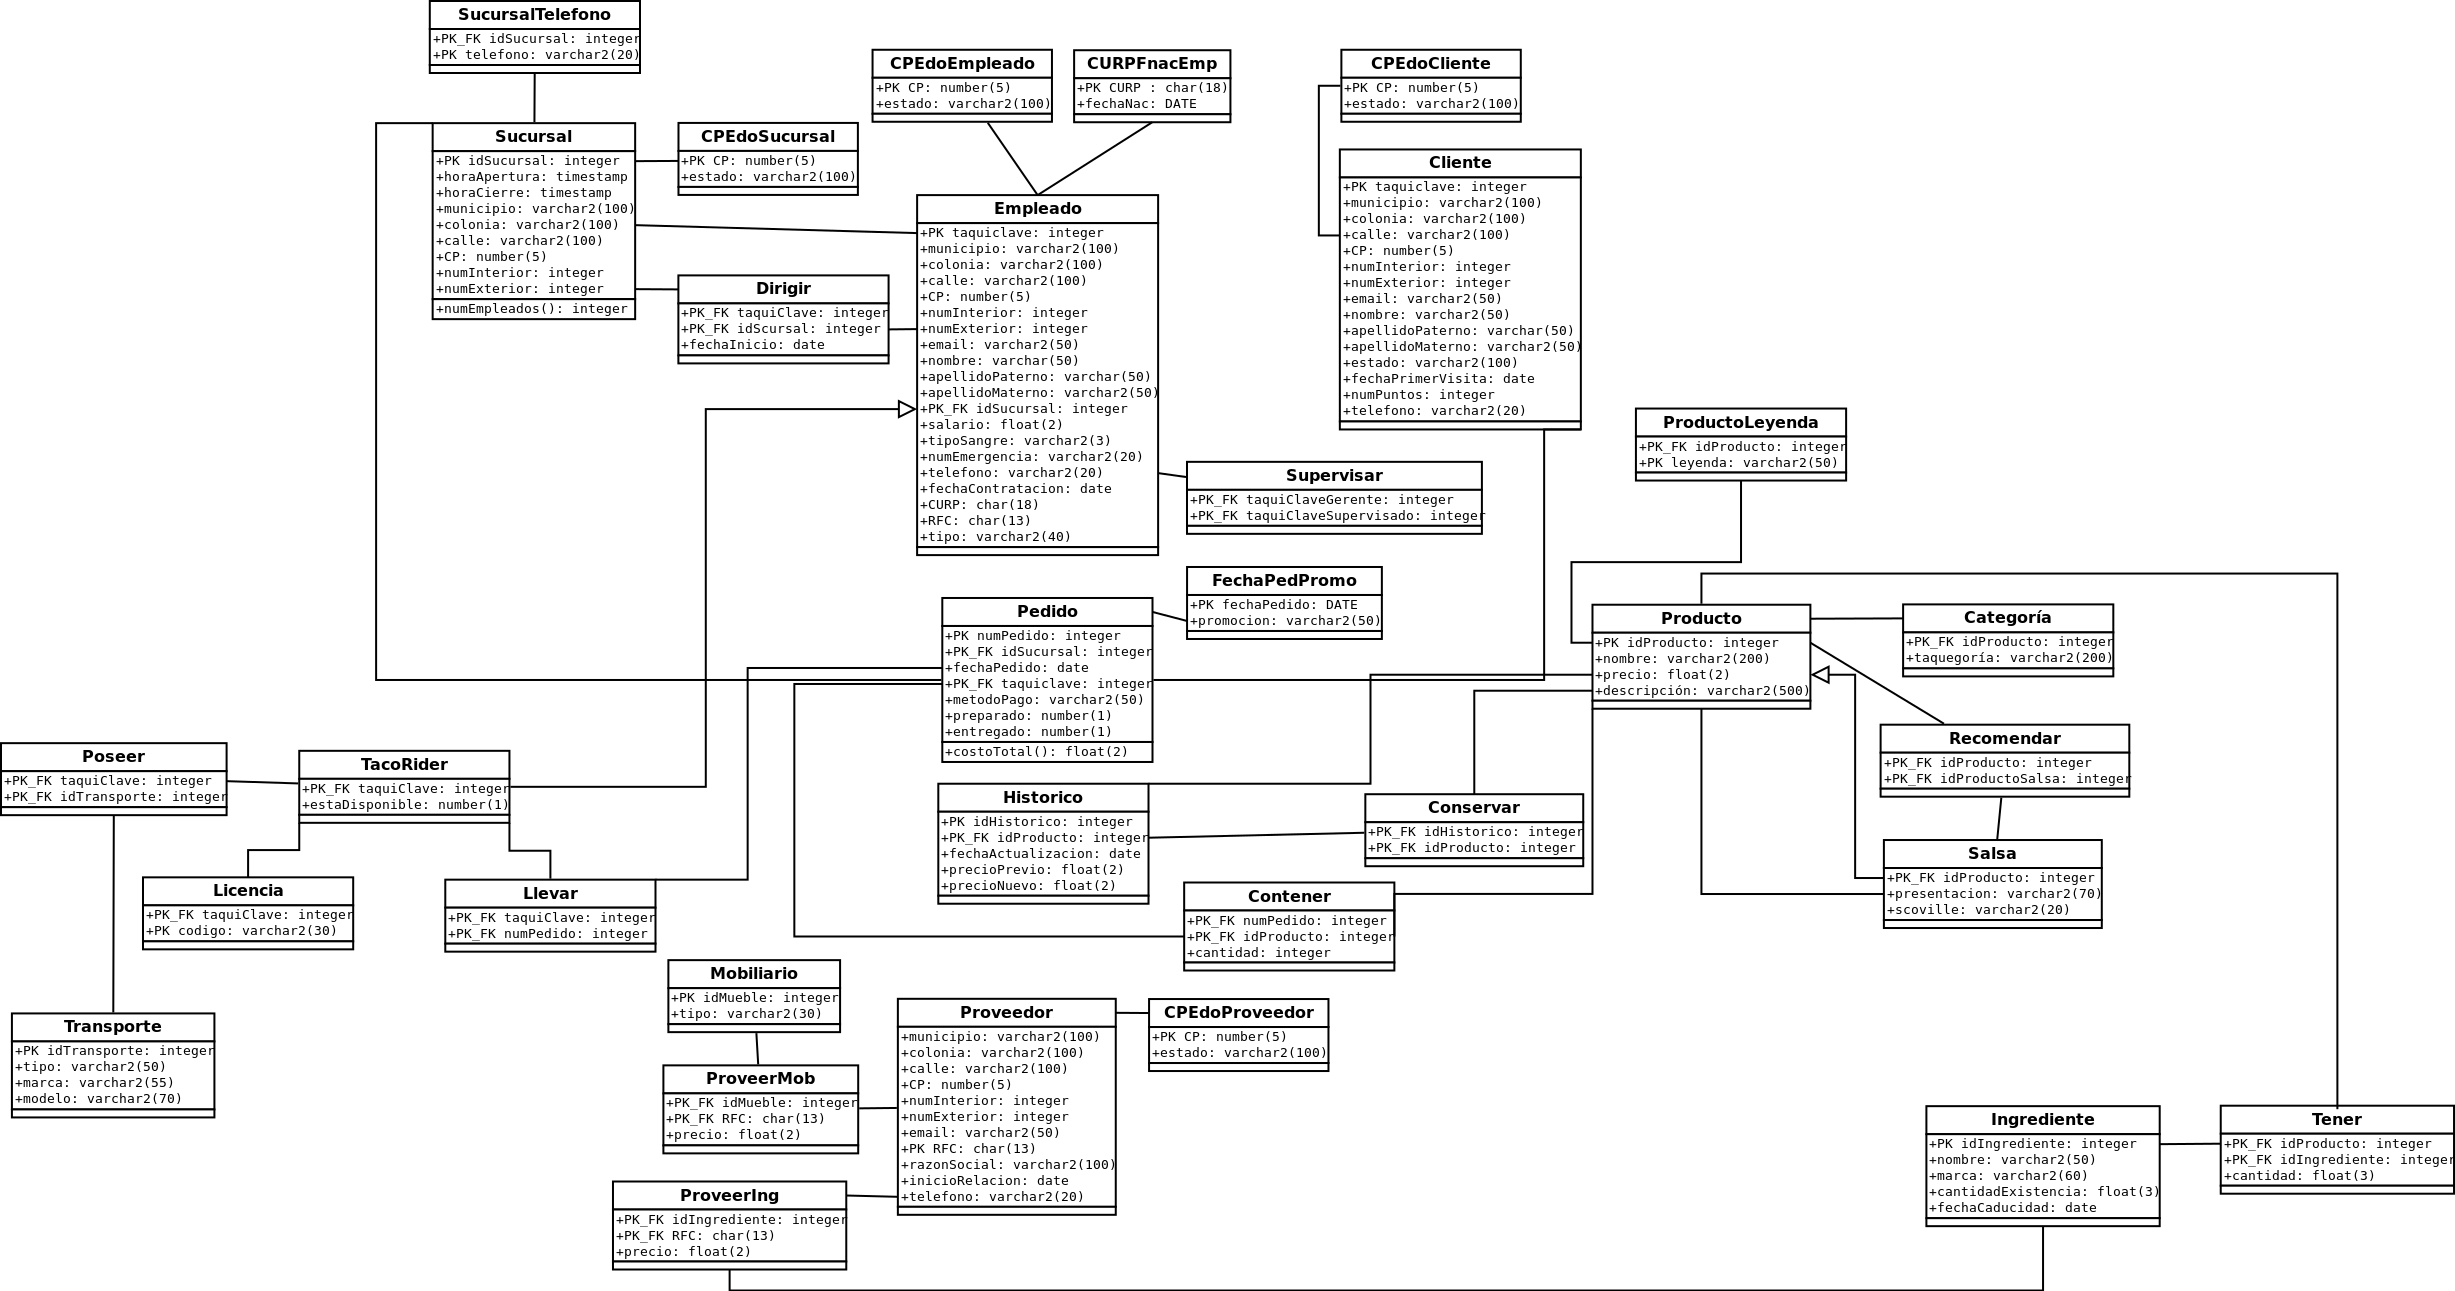
\includegraphics[width=\linewidth]{UML_normalizado.png}
\captionof{figure}{Modelo en tercera forma normal (coincidió con el de BCNF).}
\end{minipage}
\end{center}
\end{landscape}





\newpage 
 \begin{thebibliography}{1}


    \bibitem{notes} \textit{Normalización}, Avilés Rosas Gerardo. UNAM, Facultad de Ciencias, págs. 1-51.


  \end{thebibliography}
\end{document}